\chapter{7 TeV and 8 TeV Differential Cross Section Measurement: Fitting, Unfolding and Measurement}
\label{c:Differential_Cross_Section:fitting_and_unfolding}

% \section{Introduction}
% \label:{s:analysis2_introduction}
% Following event selection it is important to perform a comparison of simulation to data to verify that the
% processes modelled as backgrounds 

\section{Data-MC Comparison}
\label{ss:data-mc_comparison}
Following the full event selection, the simulated events are scaled to match the luminosity of the data using
the following scale factor:
\begin{equation}
  S = \frac{{\cal L} \times  \sigma}{N_{\rm processed}}
\end{equation}
where $N_{\rm processed}$ is the total number of events processed for each Monte Carlo sample and $\sigma$ is
the production cross section of each process. The numbers of events passing each selection step in data and
in Monte Carlo simulation are shown in Tables~\ref{tab:cut_flow_7TeV_electron} and
\ref{tab:cut_flow_7TeV_muon} for the electron and muon channels respectively at $\sqrt{s}=7\TeV$, and in
Tables~\ref{tab:cut_flow_8TeV_electron} and \ref{tab:cut_flow_8TeV_muon} for the electron and muon channels
respectively at $\sqrt{s}=8\TeV$.

\begin{table}
  \centering
   \caption{Expected and observed event yields at several stages of the electron-plus-jets selection. 
   The figures in italics are data-driven estimates of QCD background.}
    \label{tab:cut_flow_7TeV_electron}
     \resizebox{\columnwidth}{!} {
    \begin{tabular}{lrrrrrrr}
    \hline
    \hline

Selection step & \ttbar & W + Jets & Z + Jets & Single-top & QCD~  & Sum MC & Data\\
& & &  &  & Multijet &  & \\
\hline
Skim &  \\ 
Cleaning and HLT & \\ 
one isolated $e$ & \\ 
loose $e$ veto & \\ 
loose $\mu$ veto & \\ 
conversion veto & \\ 
$\geq$ 1 jets & \\
$\geq$ 2 jets & \\
$\geq$ 3 jets & \\
$\geq$ 4 jets &\\
$\geq$1 CSV \btag & \\
$\geq$2 CSV \btag & \\
\hline
\hline

    \end{tabular}
    }
\end{table}
\begin{table}
  \centering
   \caption{Expected and observed event yields at several stages of the electron-plus-jets selection. 
   The figures in italics are data-driven estimates of QCD background.}
    \label{tab:cut_flow_7TeV_muon}
     \resizebox{\columnwidth}{!} {
    \begin{tabular}{lrrrrrrr}
    \hline
    \hline

Selection step & \ttbar & W + Jets & Z + Jets & Single-top & QCD~  & Sum MC & Data\\
& & &  &  & Multijet &  & \\
\hline
Skim &  \\ 
Cleaning and HLT & \\ 
one isolated $\mu$ & \\ 
loose $\mu$ veto & \\ 
loose $e$ veto & \\ 
$\geq$ 1 jets & \\
$\geq$ 2 jets & \\
$\geq$ 3 jets & \\
$\geq$ 4 jets &\\
$\geq$1 CSV b-tag & \\
$\geq$2 CSV b-tag & \\
\hline
\hline

    \end{tabular}
    }
\end{table}
\begin{table}
  \centering
   \caption{Expected and observed event yields at several stages of the electron-plus-jets selection. 
   The figures in italics are data-driven estimates of QCD background.}
    \label{tab:cut_flow_8TeV_electron}
     \resizebox{\columnwidth}{!} {
    \begin{tabular}{lrrrrrrr}
    \hline
    \hline

Selection step & \ttbar & W + Jets & Z + Jets & Single-top & QCD~  & Sum MC & Data\\
& & &  &  & Multijet &  & \\
\hline
Skim &  \\ 
Cleaning and HLT & \\ 
one isolated $e$ & \\ 
loose $e$ veto & \\ 
loose $\mu$ veto & \\ 
conversion veto & \\ 
$\geq$ 1 jets & \\
$\geq$ 2 jets & \\
$\geq$ 3 jets & \\
$\geq$ 4 jets &\\
$\geq$1 CSV \btag & \\
$\geq$2 CSV \btag & \\
\hline
\hline

    \end{tabular}
    }
\end{table}
\begin{table}
  \centering
   \caption{Expected and observed event yields at several stages of the electron-plus-jets selection. 
   The figures in italics are data-driven estimates of QCD background.}
    \label{tab:cut_flow_8TeV_muon}
     \resizebox{\columnwidth}{!} {
    \begin{tabular}{lrrrrrrr}
    \hline
    \hline

Selection step & \ttbar & W + Jets & Z + Jets & Single-top & QCD~  & Sum MC & Data\\
& & &  &  & Multijet &  & \\
\hline
Skim &  \\ 
Cleaning and HLT & \\ 
one isolated & \\ 
loose $\mu$ veto & \\ 
loose $e$ veto & \\ 
$\geq$ 1 jets & \\
$\geq$ 2 jets & \\
$\geq$ 3 jets & \\
$\geq$ 4 jets &\\
$\geq$1 CSV b-tag & \\
$\geq$2 CSV b-tag & \\
\hline
\hline

    \end{tabular}
    }
\end{table}

The distributions of the primary variables \met, \HT, \st, \wpt and \mt after the full selection requirements
are applied are shown in Figures \ref{fig:data_mc_comparison_7TeV_electron} and
\ref{fig:data_mc_comparison_7TeV_muon} for the electron and muon channels respectively at $\sqrt{s}=7\TeV$;
and in Figures \ref{fig:data_mc_comparison_8TeV_electron} and \ref{fig:data_mc_comparison_8TeV_muon}
respectively at $\sqrt{s}=8\TeV$. The normalisations and shapes are all obtained form simulation except in the
case of QCD which is taken from data: the conversion region is used in the electron channel and the
non-isolated region is used in the muon channel. In general, the agreement between data and simulation is
good, with the distributions simulation peaking at slightly higher energies because event reweighting to
account for the \pt mismodelling of the top quark in simulation has not yet been carried out at this stage.

\begin{figure}[hbtp]
    \centering
     \includegraphics[width=0.48\textwidth]{Chapters/04_Analysis/04b_XSections/images/control_plots/before_fit/7TeV/EPlusJets_patType1CorrectedPFMet_2orMoreBtags_with_ratio.pdf}\hfill
     \includegraphics[width=0.48\textwidth]{Chapters/04_Analysis/04b_XSections/images/control_plots/before_fit/7TeV/EPlusJets_HT_2orMoreBtags_with_ratio.pdf}\\
     \includegraphics[width=0.48\textwidth]{Chapters/04_Analysis/04b_XSections/images/control_plots/before_fit/7TeV/EPlusJets_patType1CorrectedPFMet_ST_2orMoreBtags_with_ratio.pdf}\hfill
     \includegraphics[width=0.48\textwidth]{Chapters/04_Analysis/04b_XSections/images/control_plots/before_fit/7TeV/EPlusJets_patType1CorrectedPFMet_WPT_2orMoreBtags_with_ratio.pdf}\\
     \includegraphics[width=0.48\textwidth]{Chapters/04_Analysis/04b_XSections/images/control_plots/before_fit/7TeV/EPlusJets_patType1CorrectedPFMet_MT_2orMoreBtags_with_ratio.pdf}\hfill
     \caption{Comparison of Monte Carlo simulation to data in the electron+jets channel after final
     selection at $\sqrt{s}=7\TeV$.}
     \label{fig:data_mc_comparison_7TeV_electron}
\end{figure}

\begin{figure}[hbtp]
    \centering
     \includegraphics[width=0.48\textwidth]{Chapters/04_Analysis/04b_XSections/images/control_plots/before_fit/7TeV/MuPlusJets_patType1CorrectedPFMet_2orMoreBtags_with_ratio.pdf}\hfill
     \includegraphics[width=0.48\textwidth]{Chapters/04_Analysis/04b_XSections/images/control_plots/before_fit/7TeV/MuPlusJets_HT_2orMoreBtags_with_ratio.pdf}\\
     \includegraphics[width=0.48\textwidth]{Chapters/04_Analysis/04b_XSections/images/control_plots/before_fit/7TeV/MuPlusJets_patType1CorrectedPFMet_ST_2orMoreBtags_with_ratio.pdf}\hfill
     \includegraphics[width=0.48\textwidth]{Chapters/04_Analysis/04b_XSections/images/control_plots/before_fit/7TeV/MuPlusJets_patType1CorrectedPFMet_WPT_2orMoreBtags_with_ratio.pdf}\\
     \includegraphics[width=0.48\textwidth]{Chapters/04_Analysis/04b_XSections/images/control_plots/before_fit/7TeV/MuPlusJets_patType1CorrectedPFMet_MT_2orMoreBtags_with_ratio.pdf}\hfill
     \caption{Comparison of Monte Carlo simulation to data in the muon+jets channel after final
     selection at $\sqrt{s}=7\TeV$.}
     \label{fig:data_mc_comparison_7TeV_muon}
\end{figure}
 
\begin{figure}[hbtp]
    \centering
     \includegraphics[width=0.48\textwidth]{Chapters/04_Analysis/04b_XSections/images/control_plots/before_fit/8TeV/EPlusJets_patType1CorrectedPFMet_2orMoreBtags_with_ratio.pdf}\hfill
     \includegraphics[width=0.48\textwidth]{Chapters/04_Analysis/04b_XSections/images/control_plots/before_fit/8TeV/EPlusJets_HT_2orMoreBtags_with_ratio.pdf}\\
     \includegraphics[width=0.48\textwidth]{Chapters/04_Analysis/04b_XSections/images/control_plots/before_fit/8TeV/EPlusJets_patType1CorrectedPFMet_ST_2orMoreBtags_with_ratio.pdf}\hfill
     \includegraphics[width=0.48\textwidth]{Chapters/04_Analysis/04b_XSections/images/control_plots/before_fit/8TeV/EPlusJets_patType1CorrectedPFMet_WPT_2orMoreBtags_with_ratio.pdf}\\
     \includegraphics[width=0.48\textwidth]{Chapters/04_Analysis/04b_XSections/images/control_plots/before_fit/8TeV/EPlusJets_patType1CorrectedPFMet_MT_2orMoreBtags_with_ratio.pdf}\hfill
     \caption{Comparison of Monte Carlo simulation to data in the electron+jets channel after final
     selection at $\sqrt{s}=8\TeV$.}
     \label{fig:data_mc_comparison_8TeV_electron}
\end{figure}
 
\begin{figure}[hbtp]
    \centering
     \includegraphics[width=0.48\textwidth]{Chapters/04_Analysis/04b_XSections/images/control_plots/before_fit/8TeV/MuPlusJets_patType1CorrectedPFMet_2orMoreBtags_with_ratio.pdf}\hfill
     \includegraphics[width=0.48\textwidth]{Chapters/04_Analysis/04b_XSections/images/control_plots/before_fit/8TeV/MuPlusJets_HT_2orMoreBtags_with_ratio.pdf}\\
     \includegraphics[width=0.48\textwidth]{Chapters/04_Analysis/04b_XSections/images/control_plots/before_fit/8TeV/MuPlusJets_patType1CorrectedPFMet_ST_2orMoreBtags_with_ratio.pdf}\hfill
     \includegraphics[width=0.48\textwidth]{Chapters/04_Analysis/04b_XSections/images/control_plots/before_fit/8TeV/MuPlusJets_patType1CorrectedPFMet_WPT_2orMoreBtags_with_ratio.pdf}\\
     \includegraphics[width=0.48\textwidth]{Chapters/04_Analysis/04b_XSections/images/control_plots/before_fit/8TeV/MuPlusJets_patType1CorrectedPFMet_MT_2orMoreBtags_with_ratio.pdf}\hfill
     \caption{Comparison of Monte Carlo simulation to data in the muon+jets channel after final
     selection at $\sqrt{s}=8\TeV$.}
     \label{fig:data_mc_comparison_8TeV_muon}
\end{figure}

A comparison between data and simulation in the electron+jets QCD selections is shown in
Figure~\ref{fig:data_mc_comparison_electron_QCD}. There is reasonably good agreement between the data and
simulation in the conversion selection but low statistics in the $\sqrt{s}=8\TeV$ simulation lead to some
events with large weights, leading to peaks in the distribution. It can also be seen that there are more
conversion events in the regions of the endcaps, where the larger amount of detector material for electrons to
traverse leads to a higher number of conversions. The non-isolated QCD selection shows more discrepancies
between the simulation and data, but it should be noted that at $\sqrt{s}=7\TeV$ the simulation does not
contain the triggers used in this analysis, unlike at $\sqrt{s}=8\TeV$, therefore the simulation distirbution
at $\sqrt{s}=7\TeV$ is not affected by the trigger isolation requirements.

The true QCD background distribution is a mixture of the conversion and non-isolated distributions. A
comparison of the two QCD background selections at $\sqrt{s}=7\TeV$ and $\sqrt{s}=8\TeV$ is also shown in the
lower plots in Figure~\ref{fig:data_mc_comparison_electron_QCD}. Background events in which electrons come
from jets misreconstructed as electrons or from \bquark or \cquark decays will pass the non-isolated
selection, whereas conversion events in which the second electron is not rejected by the electron veto will
pass the conversion selection. Another point to note is that, while the general shape of the conversion
selection is expected to be the same in both signal and QCD background selections, the same may not be true of
the non-isolated selection due to the isolation requirement in the signal selection. In addition, the number
of events passing the QCD background selections will be very small compared to the number of events passing
the signal selection, so the effect of even large uncertainties in the QCD background on the total number of
events will be minimal.

In the muon+jets channel, again it is clear that the data and simulation are not in agreement and that there
is a low amount of statistics available in simulation.

 \begin{figure}[hbtp]
    \centering
%      \includegraphics[width=0.48\textwidth]{Chapters/04_Analysis/04b_XSections/images/control_plots/before_fit/7TeV/}\hfill
%      \includegraphics[width=0.48\textwidth]{Chapters/04_Analysis/04b_XSections/images/control_plots/before_fit/8TeV/}\\
%      \includegraphics[width=0.48\textwidth]{Chapters/04_Analysis/04b_XSections/images/control_plots/before_fit/7TeV/}\hfill
%      \includegraphics[width=0.48\textwidth]{Chapters/04_Analysis/04b_XSections/images/control_plots/before_fit/8TeV/}\\
%      \includegraphics[width=0.48\textwidth]{Chapters/04_Analysis/04b_XSections/images/control_plots/before_fit/7TeV/}\hfill
%      \includegraphics[width=0.48\textwidth]{Chapters/04_Analysis/04b_XSections/images/control_plots/before_fit/7TeV/}\\
     
\includegraphics[width=0.48\textwidth]{Chapters/04_Analysis/04b_XSections/images/placeholder.png}\hfill
     
\includegraphics[width=0.48\textwidth]{Chapters/04_Analysis/04b_XSections/images/placeholder.png}\\
     
\includegraphics[width=0.48\textwidth]{Chapters/04_Analysis/04b_XSections/images/placeholder.png}\hfill
     
\includegraphics[width=0.48\textwidth]{Chapters/04_Analysis/04b_XSections/images/placeholder.png}\\
     
\includegraphics[width=0.48\textwidth]{Chapters/04_Analysis/04b_XSections/images/placeholder.png}\hfill
     
\includegraphics[width=0.48\textwidth]{Chapters/04_Analysis/04b_XSections/images/placeholder.png}\\
     \caption{Comparison of QCD selections in the electron+jets channel at $\sqrt{s}=7\TeV$ on the left
     and at $\sqrt{s}=8\TeV$ on the right. Conversion region is shown at the top, non-isolated selection
     in the middle and a comparison of the two selections in data (TODO:CHECK THIS, AND INSERT THE PLOTS IN
     THE FIRST PLACE!)
     %TODO:CHECK THIS
     is shown in the lower plots.}
     \label{fig:data_mc_comparison_electron_QCD}
 \end{figure}

\section{Binning Choice}
\label{s:binning_choice}
The bin boundaries in the primary variable distributions is important because events generated in one bin can
migrate to another bin after reconstrution due to the finite resolution of the detector. This altering of the
number of events, either as a result of events moving into, or out of, a bin is important to understand so
that the final reconstructed distribution can be deconvoluted (unfolded) to the true distribution.

In light of this, the binning choice is made based on two variables defined as purity ($p^k$) and stability
($s^k$):

\begin{eqnarray}
\label{eq:purity_and_stability}
p^k = \frac{N_{\rec\&\gen}^k}{N_{\rec}^k}
s^k = \frac{N_{\rec\&\gen}^k}{N_{\gen}^k}
,
\end{eqnarray}

$N_{\rec\&\gen}^k$ is the number of events generated and reconstructed in bin $k$,
$N_{\rec}^k$ is the number of events reconstructed in bin $k$ and $N_{\gen}^k$ is the number of events
generated in bin $k$. The stability of a bin is sensitive to the migration of events out of a bin, while
the purity is sensitive to the migration of events into a bin (see Figure~\ref{fig:purity_and_stability}).

\begin{figure}[hbtp]
	\centering
     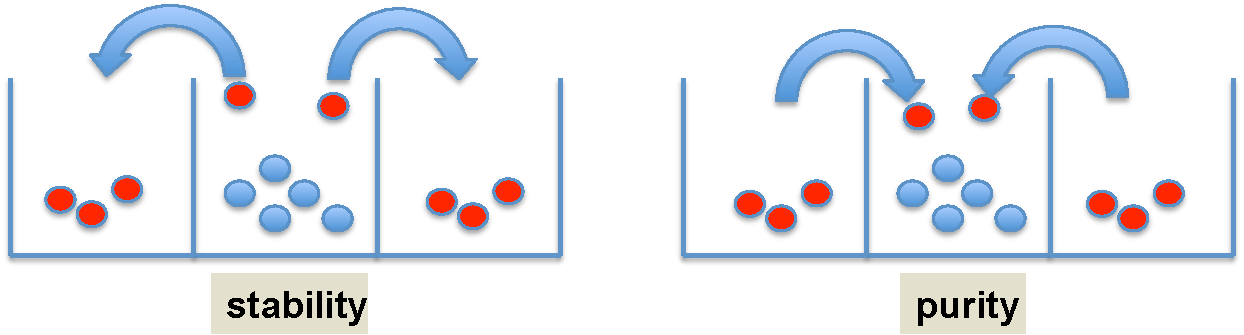
\includegraphics[width=0.8\textwidth]{Chapters/04_Analysis/04b_XSections/images/purity_and_stability.pdf}
     \caption{Stability quantifies the migration of events out of a bin while purity quantifies the migration
     of events into a bin. Both quantities compare the variable range (bin) in which an event is generated to
     the range in which they are reconstructed.}
     \label{fig:purity_and_stability}
 \end{figure}

In this analysis, the bins for each primary variable distribution were chosen such that all bins have purity
and stability values of 0.5 or greater, meaning that at least half of the events generated in a bin remain in that bin
after reconstruction, and that at least half of the events reconstructed in a bin were generated in that bin.
In order to avoid very small bins, a requirement that all bins have at least 100 events is also enforced.

The determination of the bin boundaries following these criteria is carried out simultaneously in (and
therefore the binning is identical in) both centre of mass energies and both the electron+jets and
muon+jets channel.

Plots of generated versus reconstructed events for all primary variables are shown in the electron+jets
channel in Figure~\ref{fig:binning_7TeV_electron} for $\sqrt{s}=7\TeV$ and in
Figure~\ref{fig:binning_8TeV_electron} for $\sqrt{s}=8\TeV$. The corresponding plots in the muon+jets are
shown in Figures~\ref{fig:binning_7TeV_muon} and \ref{fig:binning_8TeV_muon} in
Appendix~\ref{as:binning_muon}. The purity and stability values of the chosen bins are shown in
Appendix~\ref{as:binning_tables_electron}.

\begin{figure}[hbtp]
	\centering
     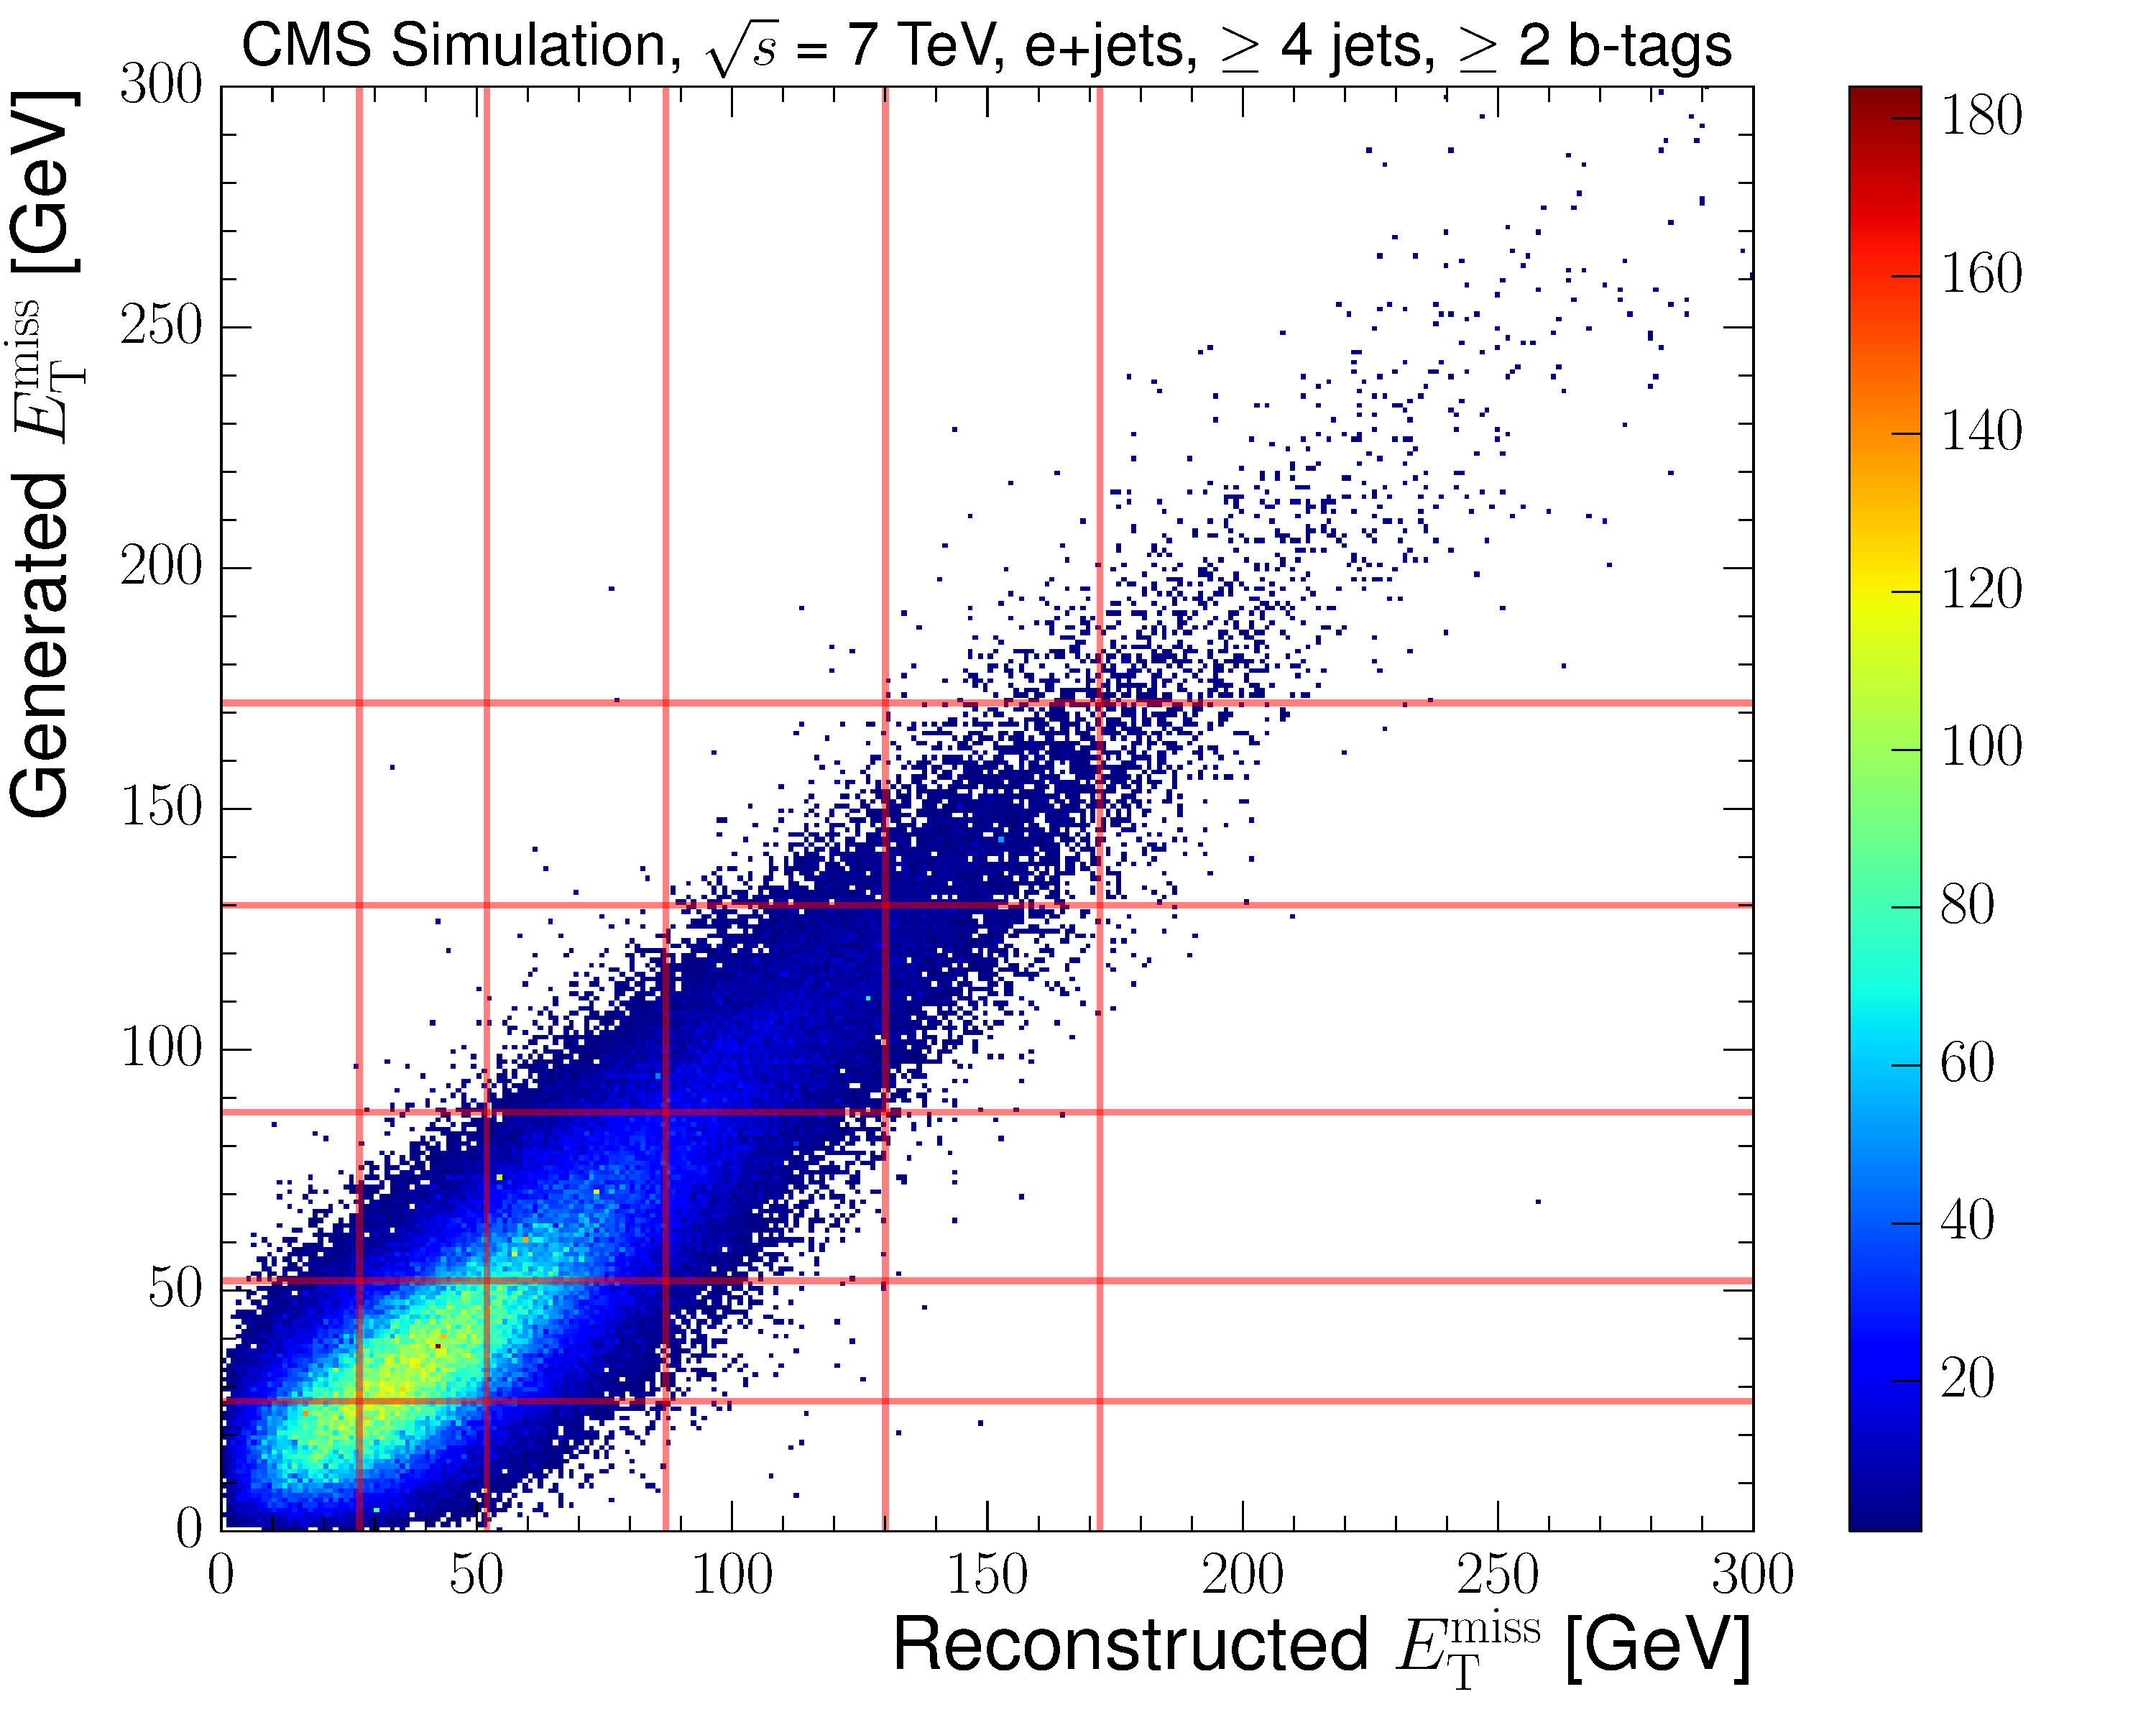
\includegraphics[width=0.48\textwidth]{Chapters/04_Analysis/04b_XSections/images/binning/electron_MET_7TeV.pdf}\hfill
     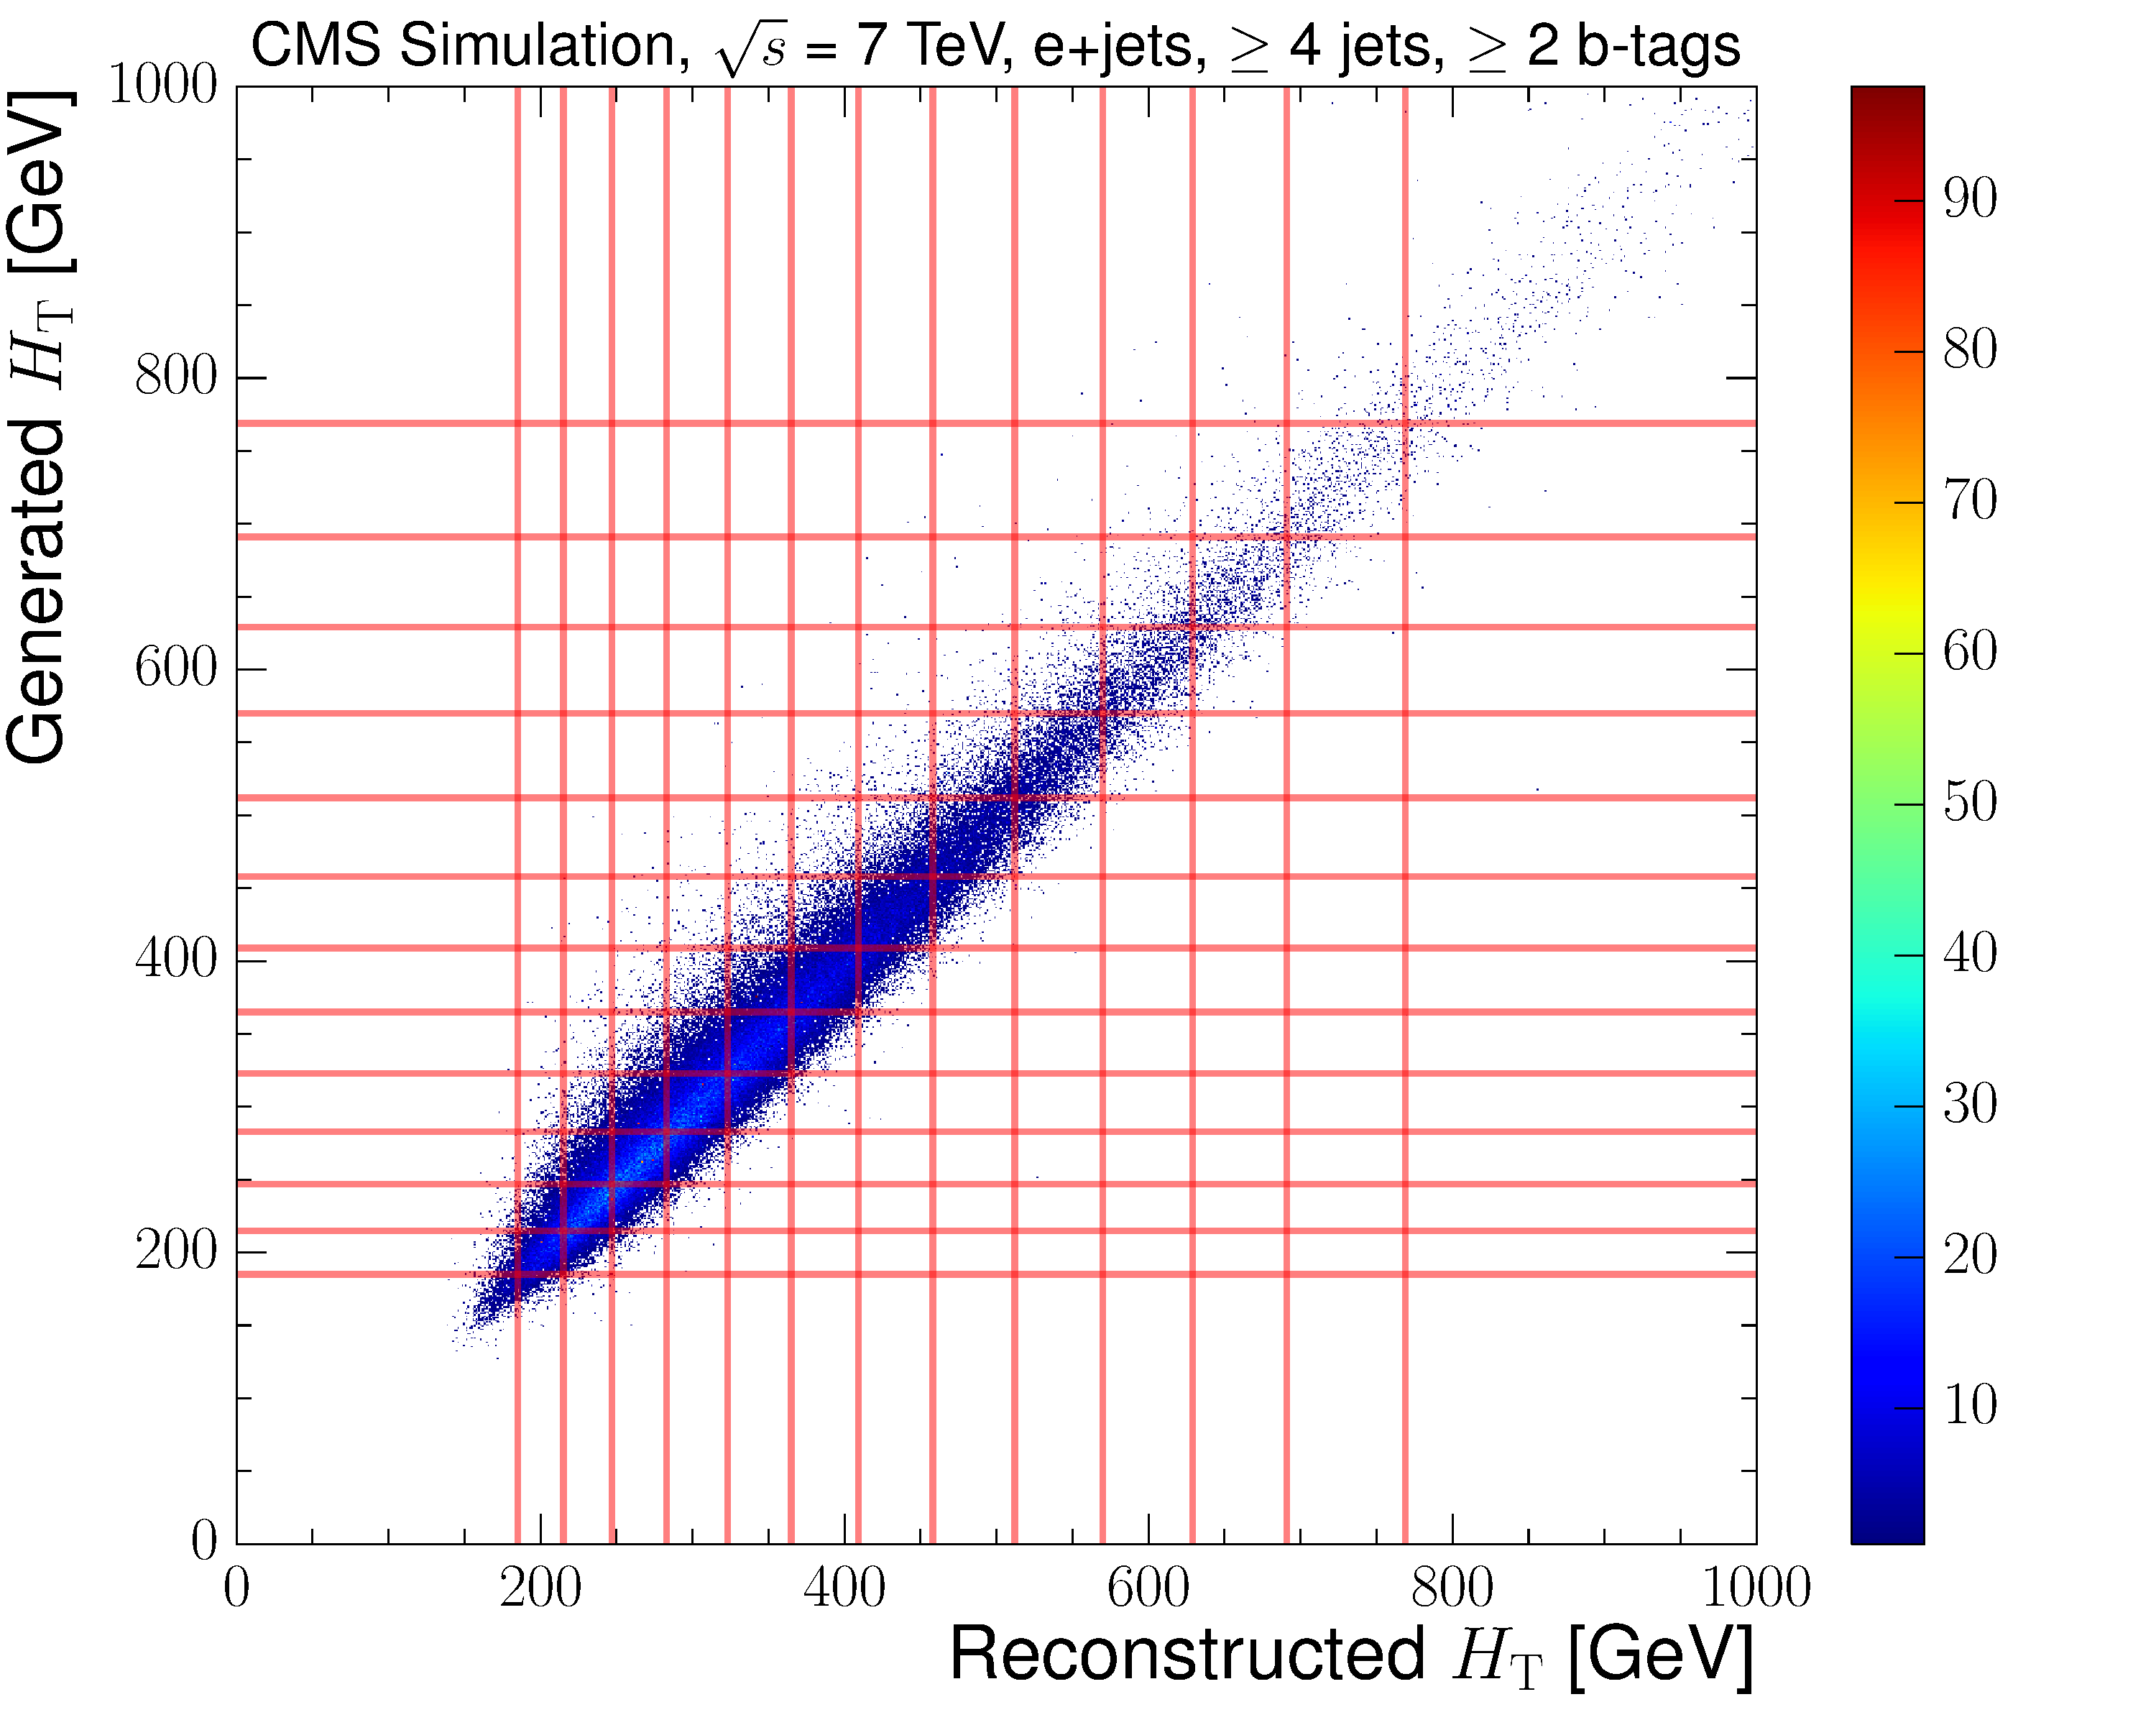
\includegraphics[width=0.48\textwidth]{Chapters/04_Analysis/04b_XSections/images/binning/electron_HT_7TeV.pdf}\\
     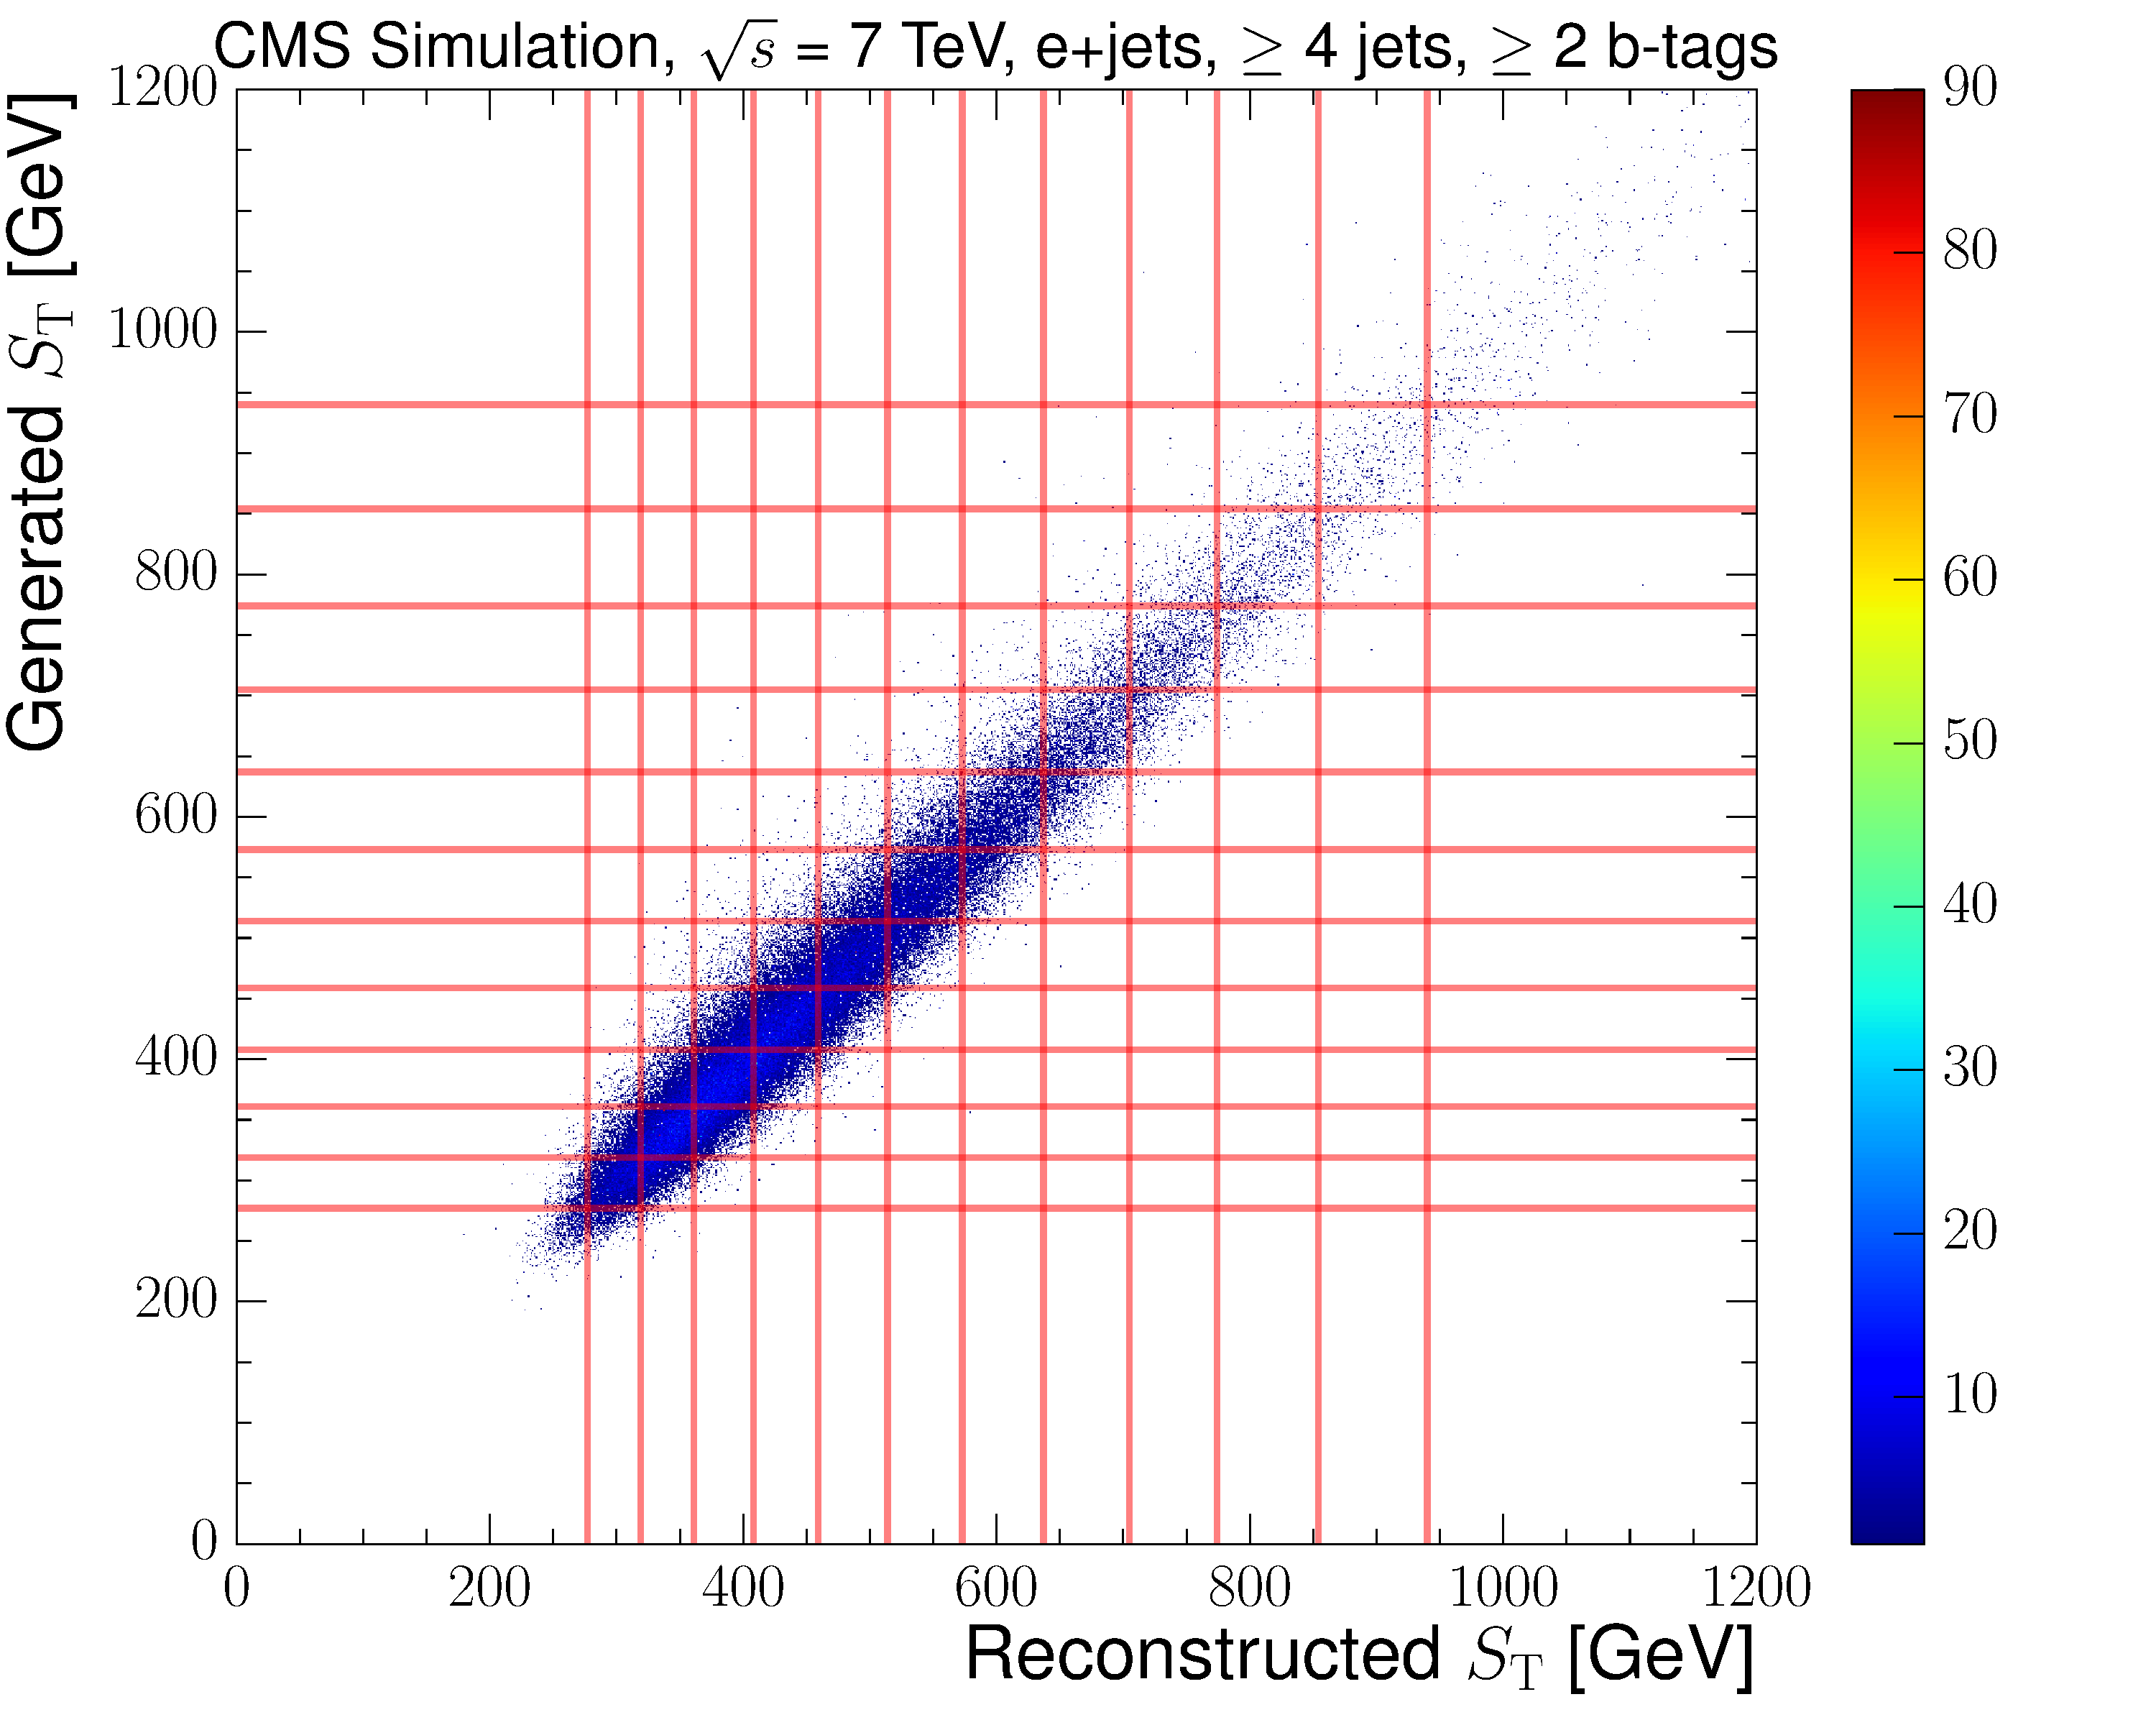
\includegraphics[width=0.48\textwidth]{Chapters/04_Analysis/04b_XSections/images/binning/electron_ST_7TeV.pdf}\hfill
     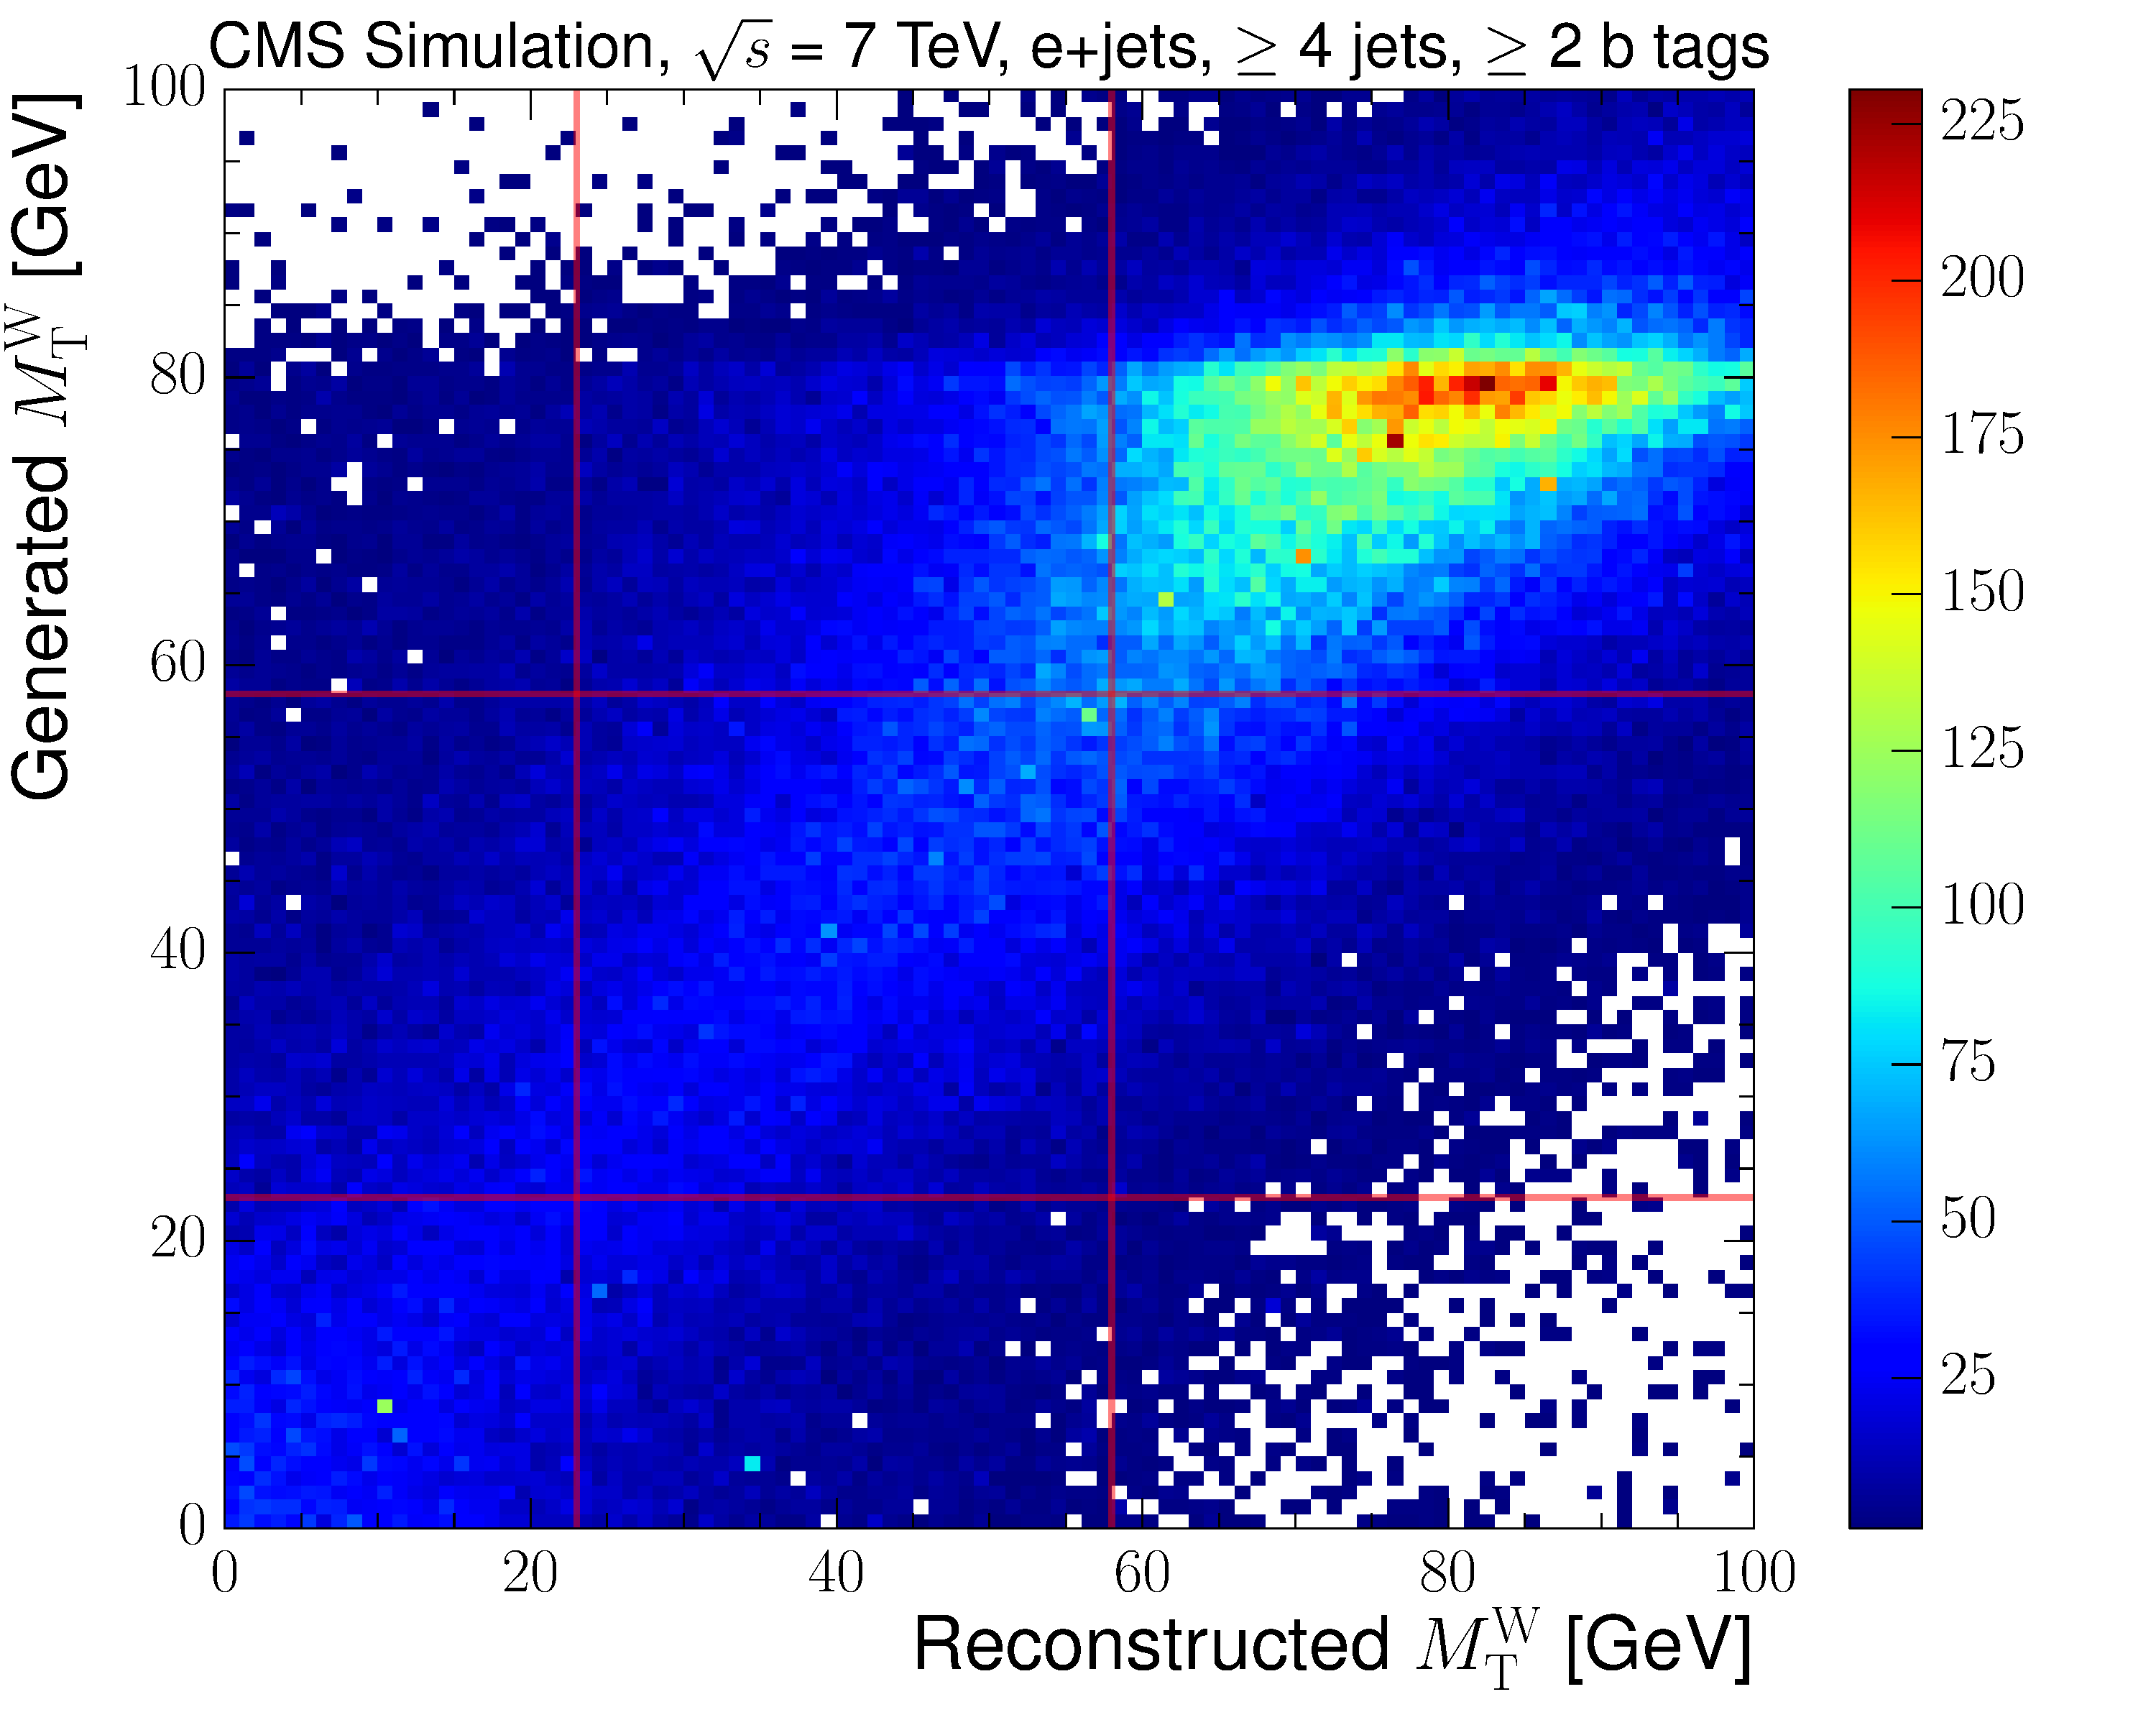
\includegraphics[width=0.48\textwidth]{Chapters/04_Analysis/04b_XSections/images/binning/electron_MT_7TeV.pdf}\\
	 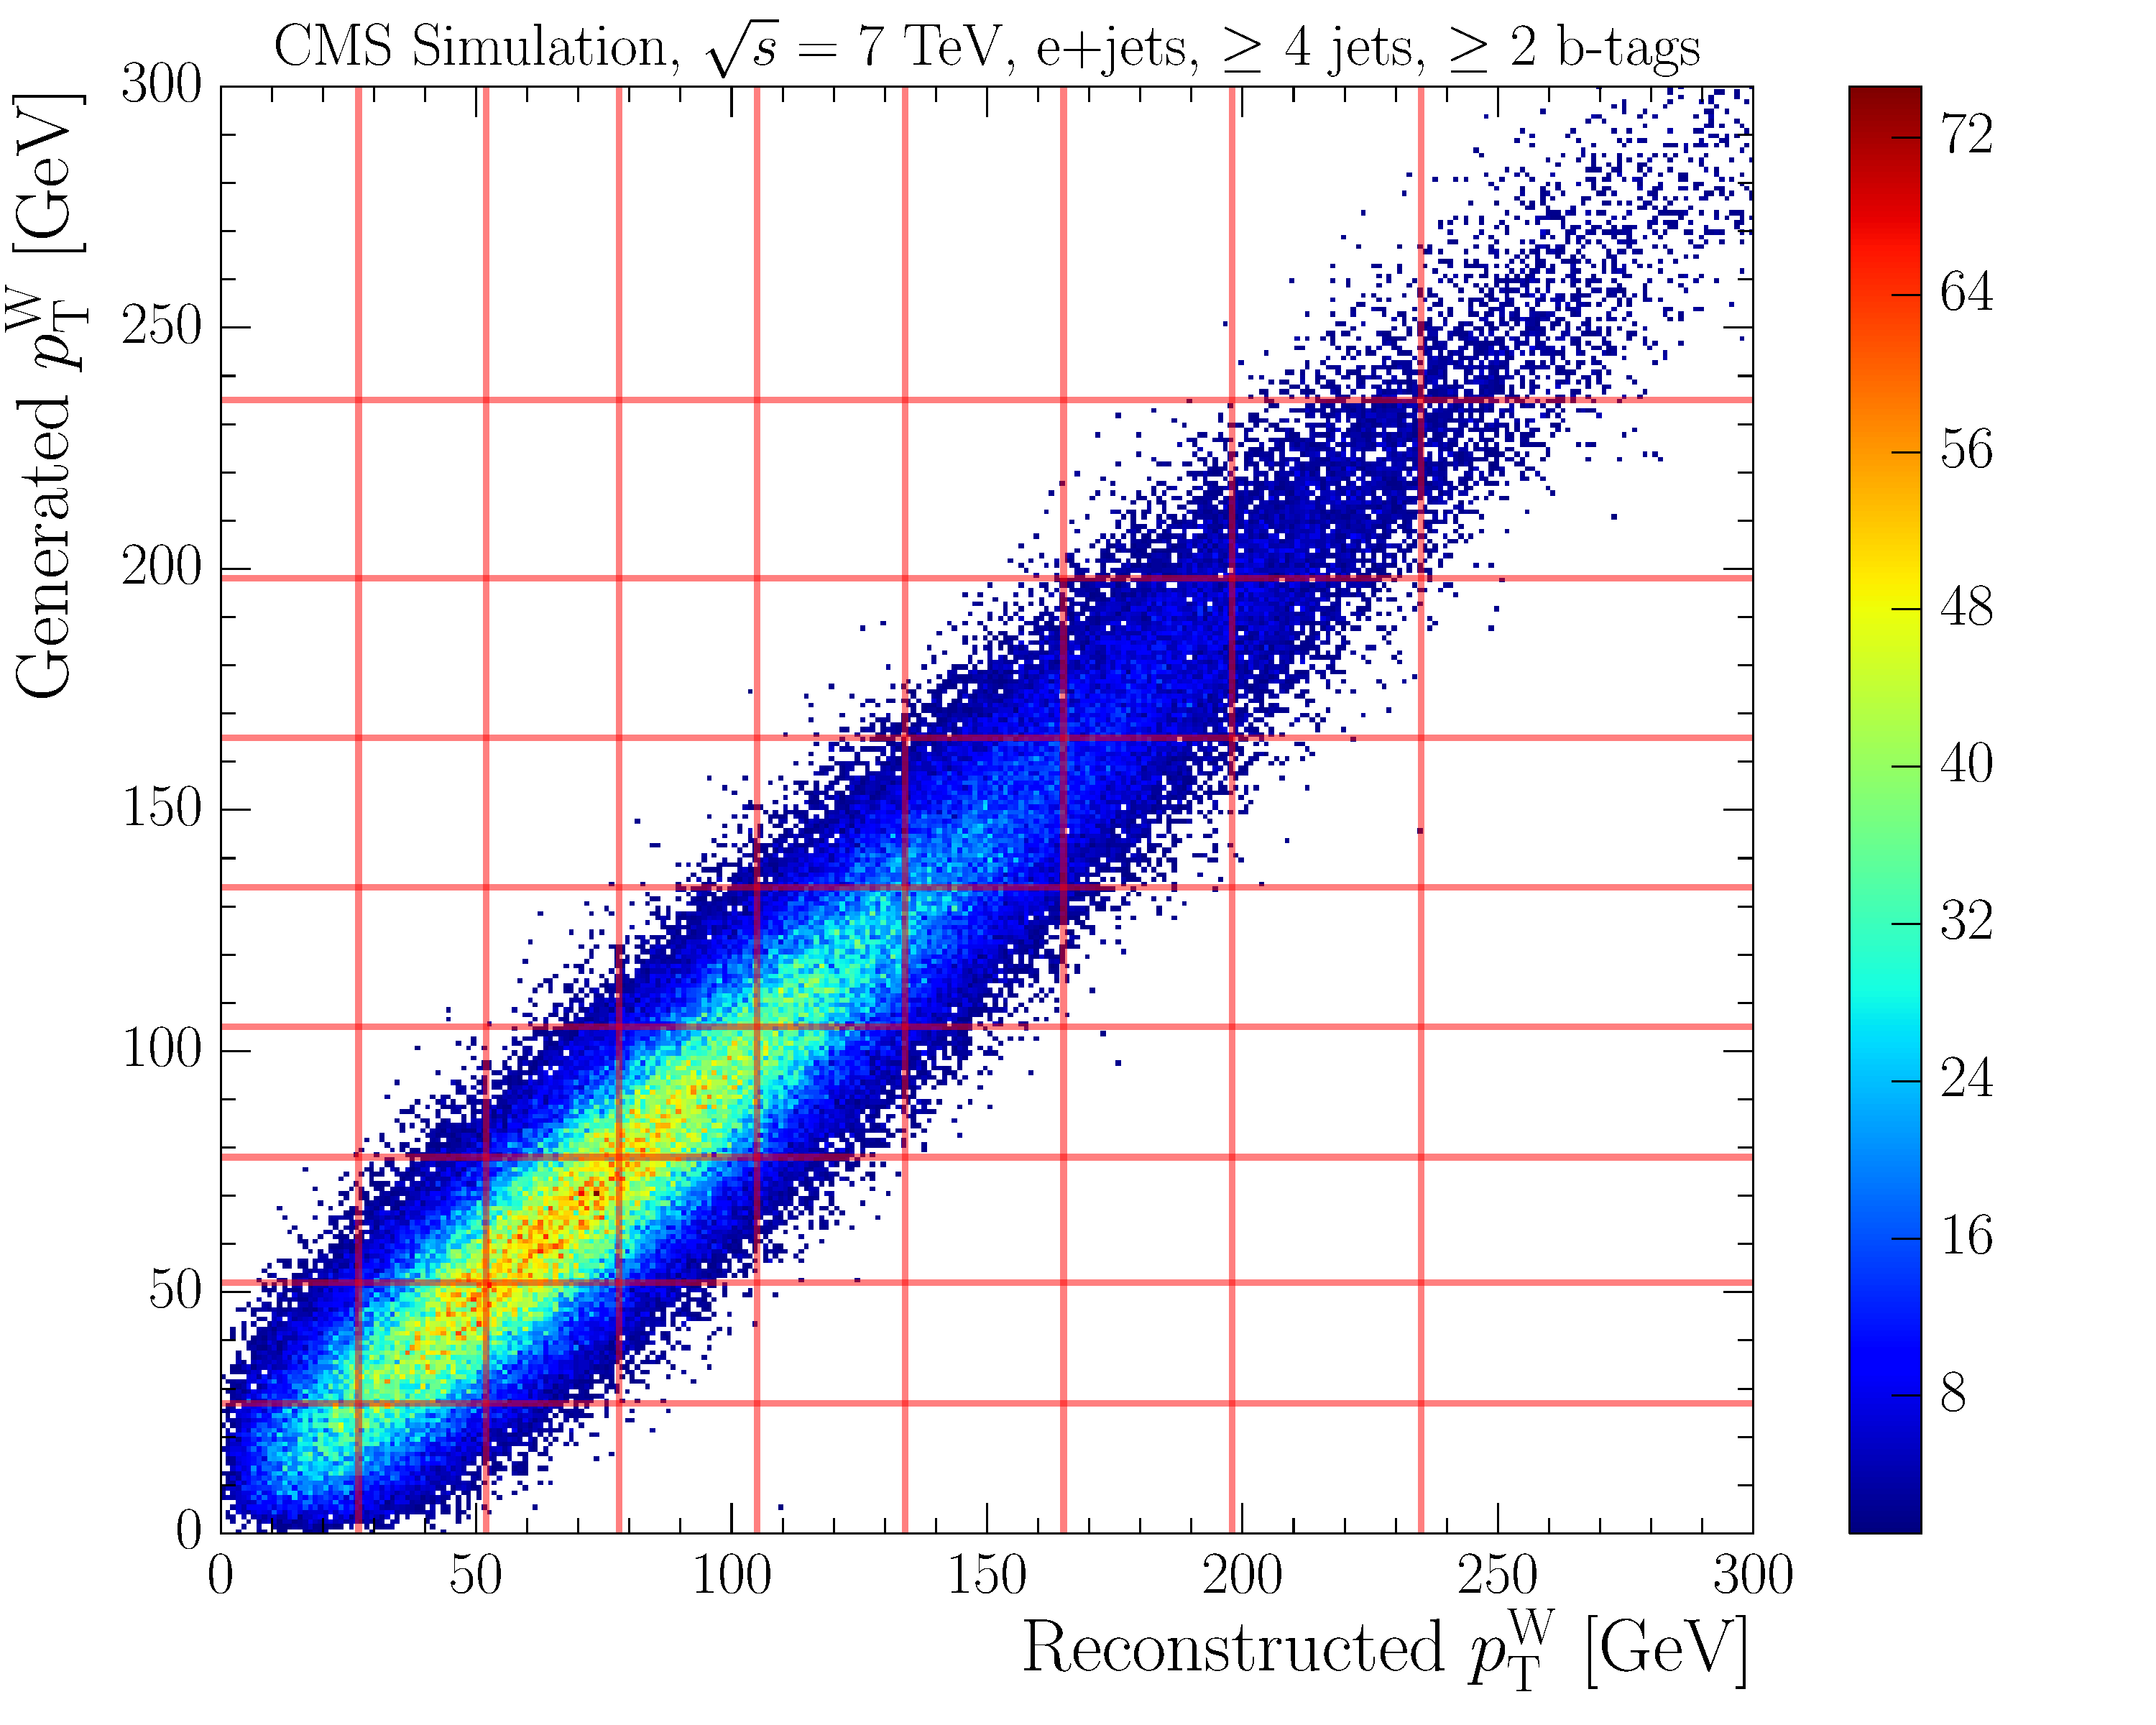
\includegraphics[width=0.48\textwidth]{Chapters/04_Analysis/04b_XSections/images/binning/electron_WPT_7TeV.pdf}\hfill
	 \caption{Generated versus reconstructed distributions of the primary variables \met (upper left), \HT (upper
	 right), \st (middle left), \mt (middle right) and \wpt (lower) with horizontal and vertical lines
	 representing the boundaries of the selected bins at $\sqrt{s}=7\TeV$ in the electron+ jets channel. These
	 distributions are obtained using \ttbar Monte Carlo simulation.}
     \label{fig:binning_7TeV_electron}
\end{figure}

\begin{figure}[hbtp]
    \centering
     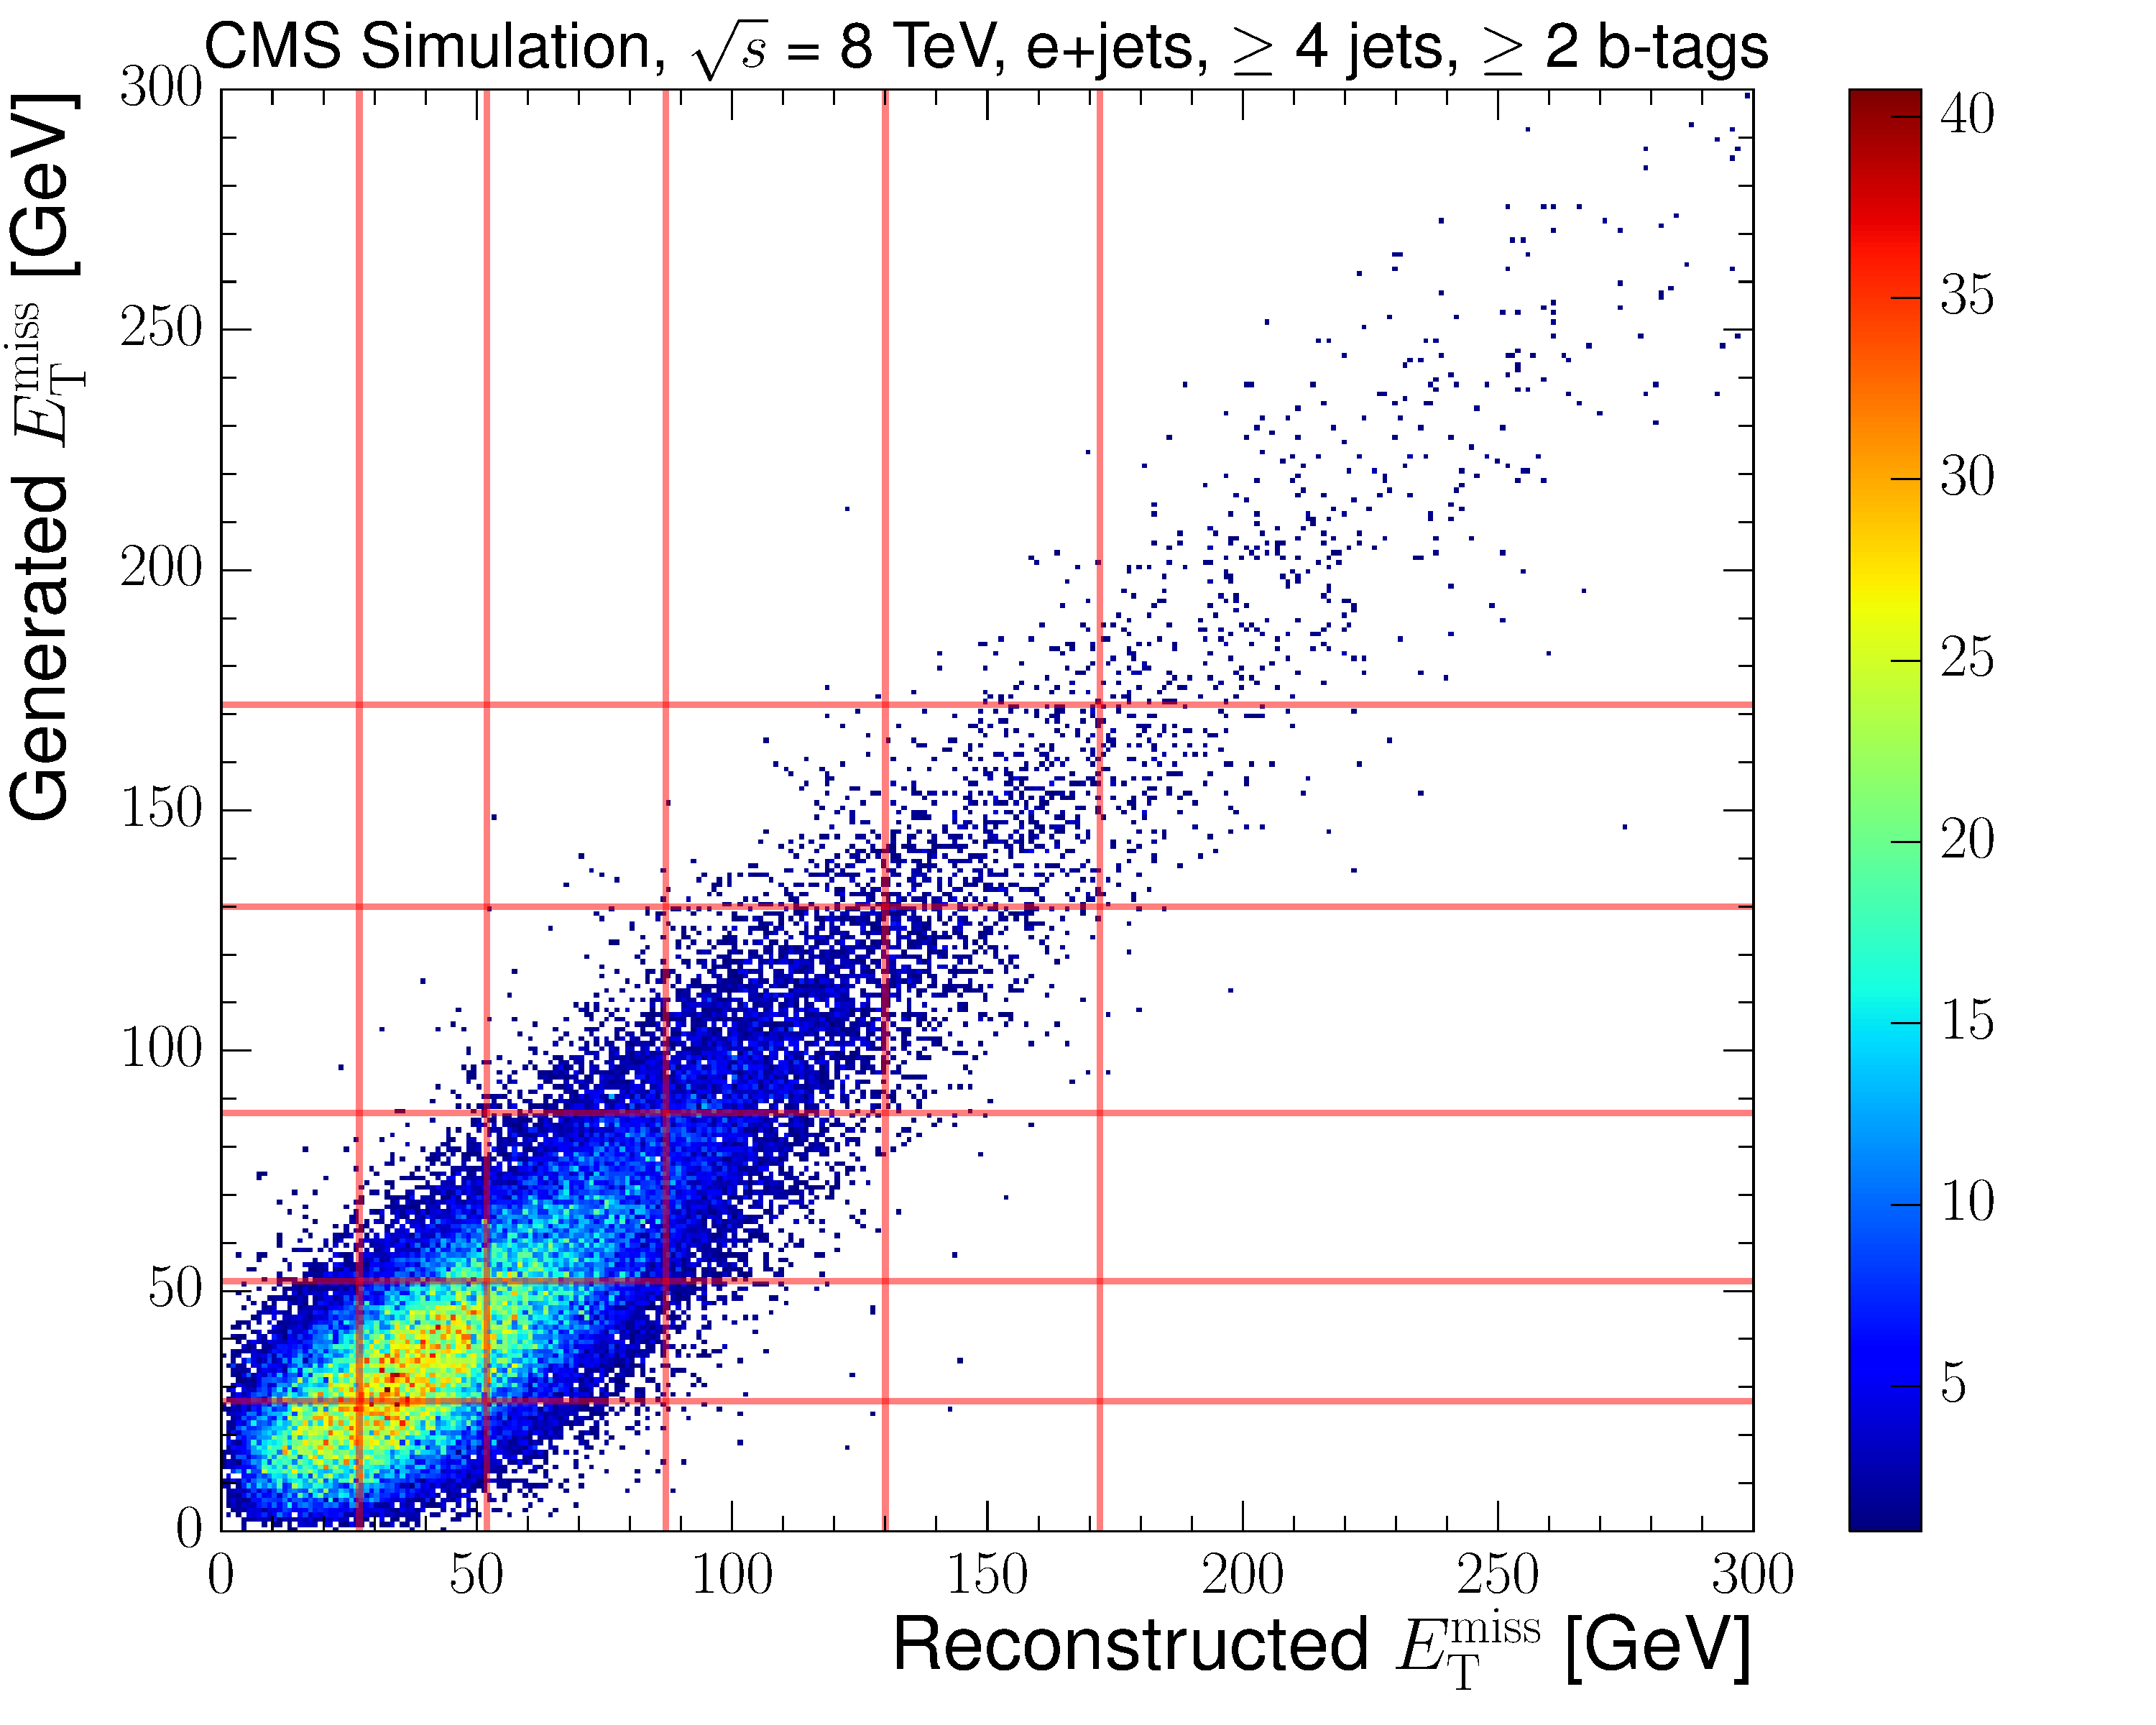
\includegraphics[width=0.48\textwidth]{Chapters/04_Analysis/04b_XSections/images/binning/electron_MET_8TeV.pdf}\hfill
     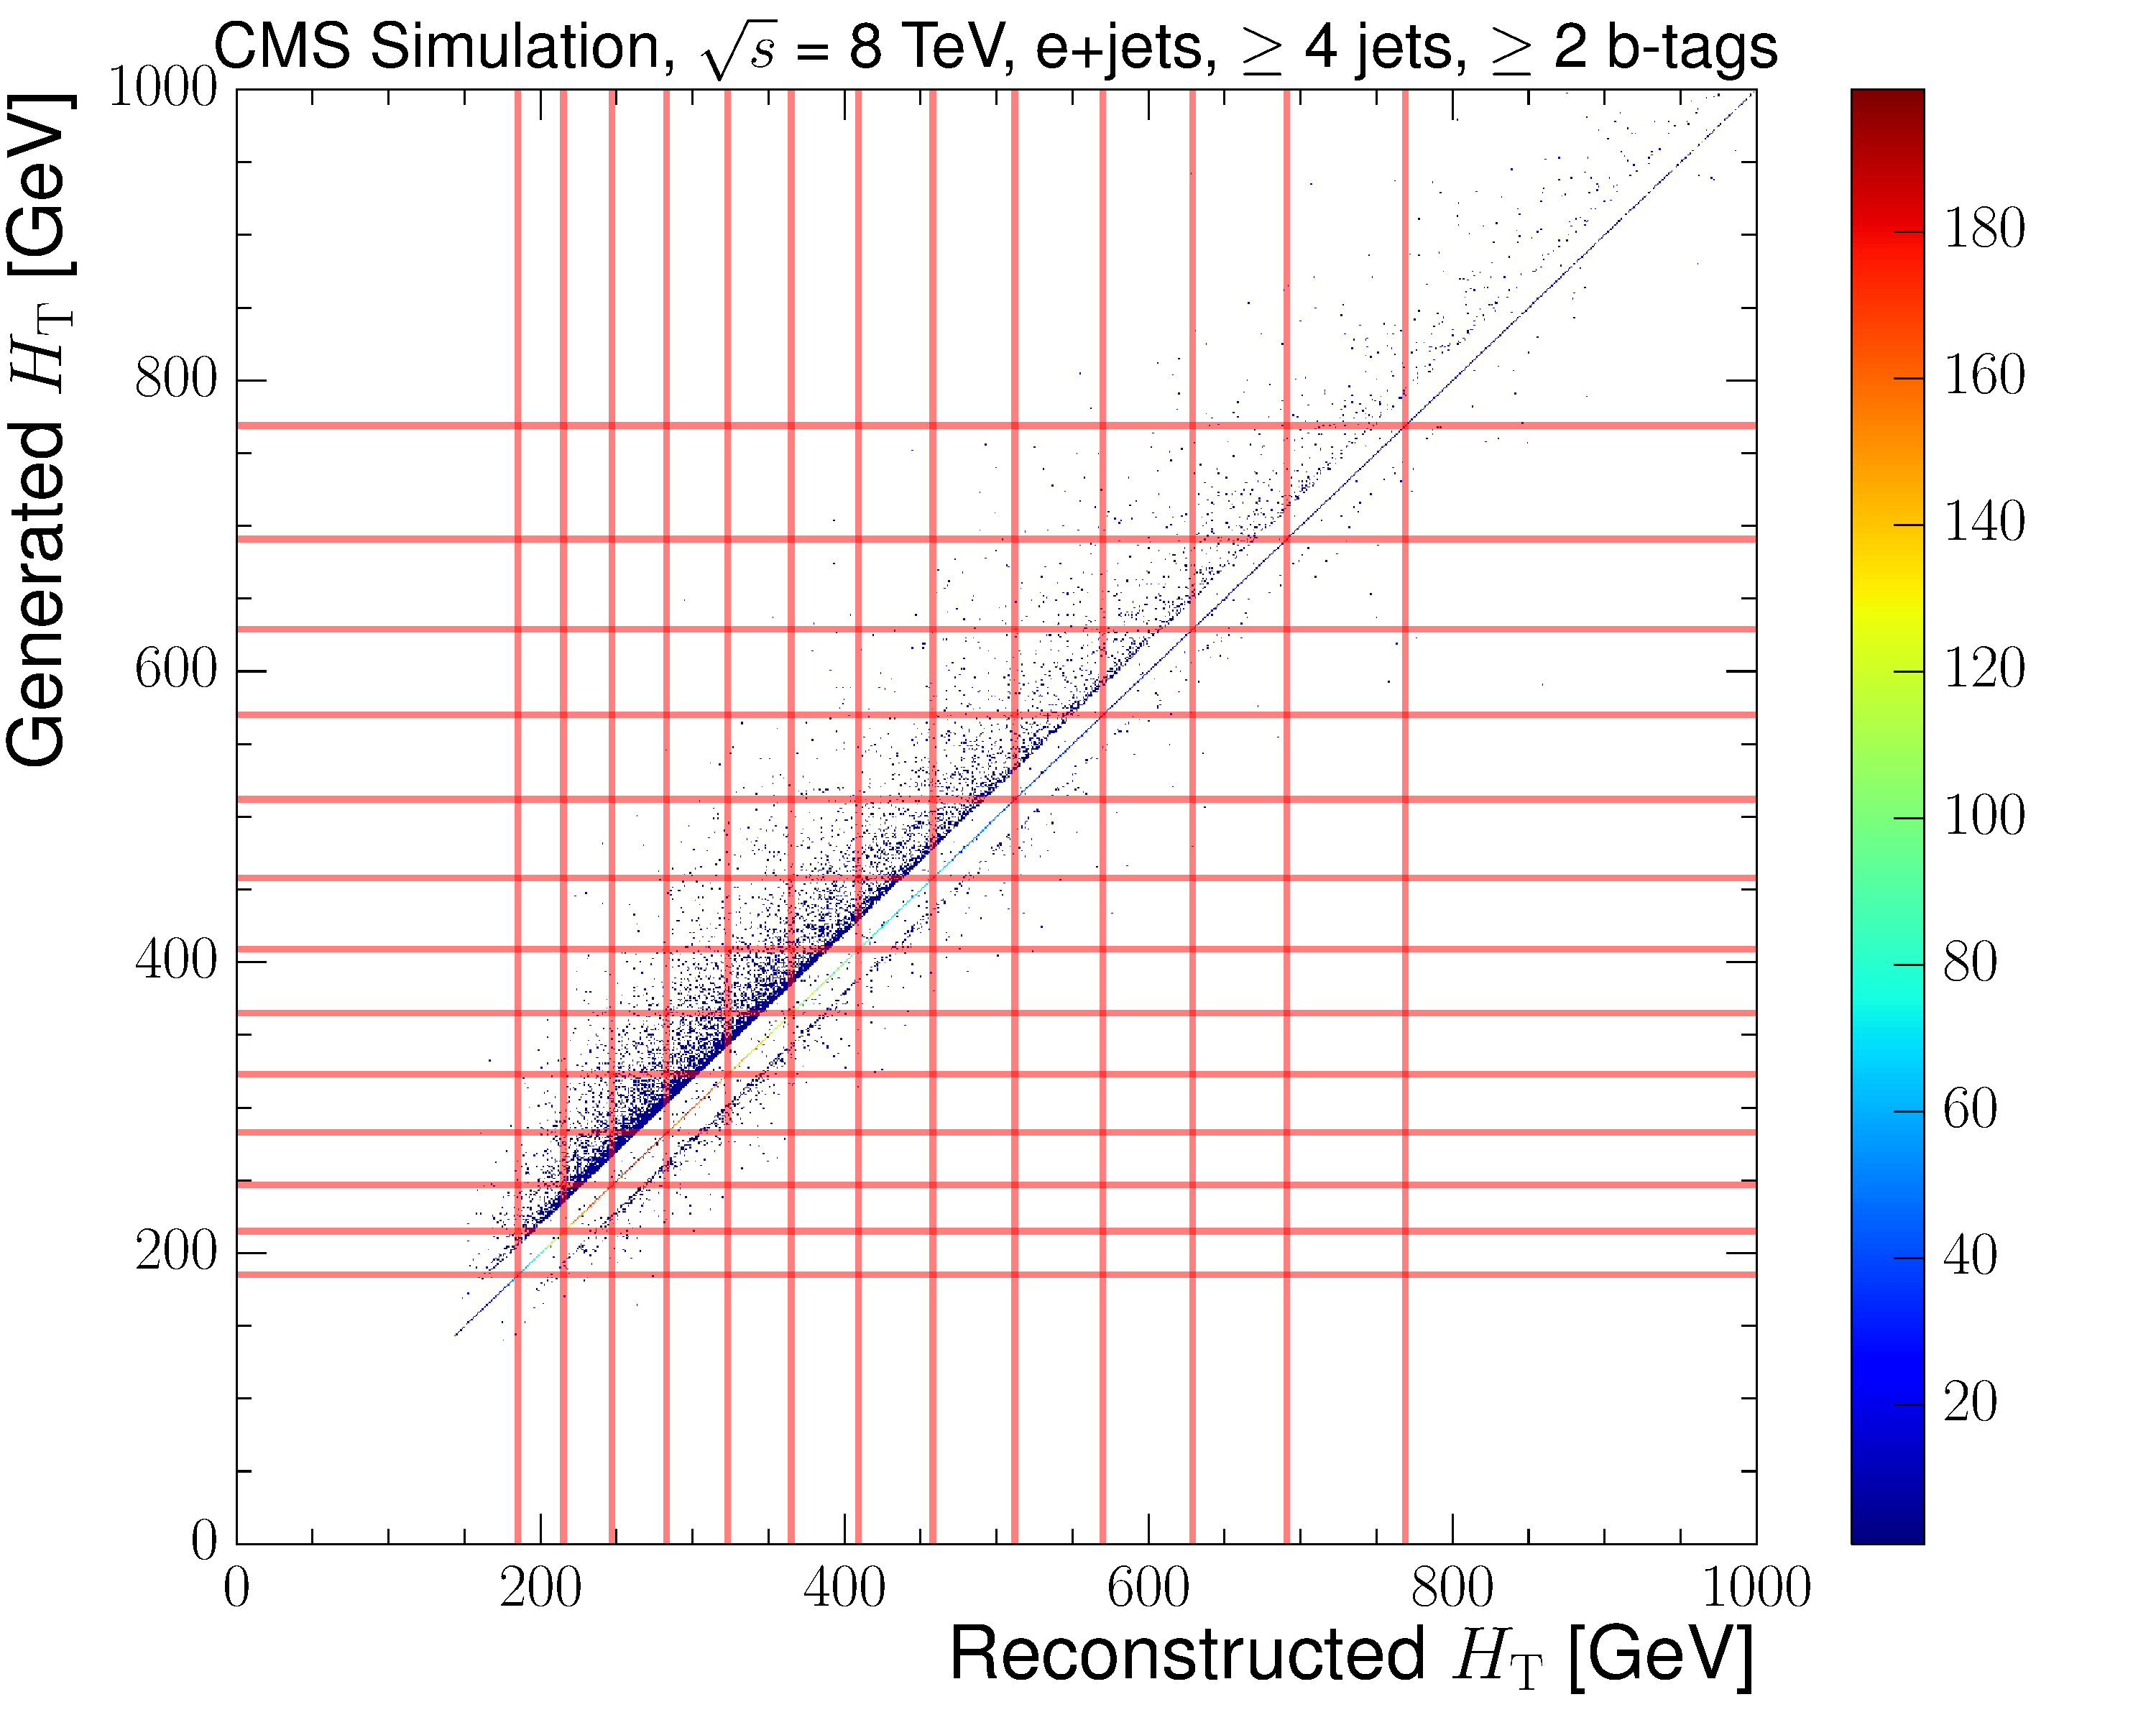
\includegraphics[width=0.48\textwidth]{Chapters/04_Analysis/04b_XSections/images/binning/electron_HT_8TeV.pdf}\\
     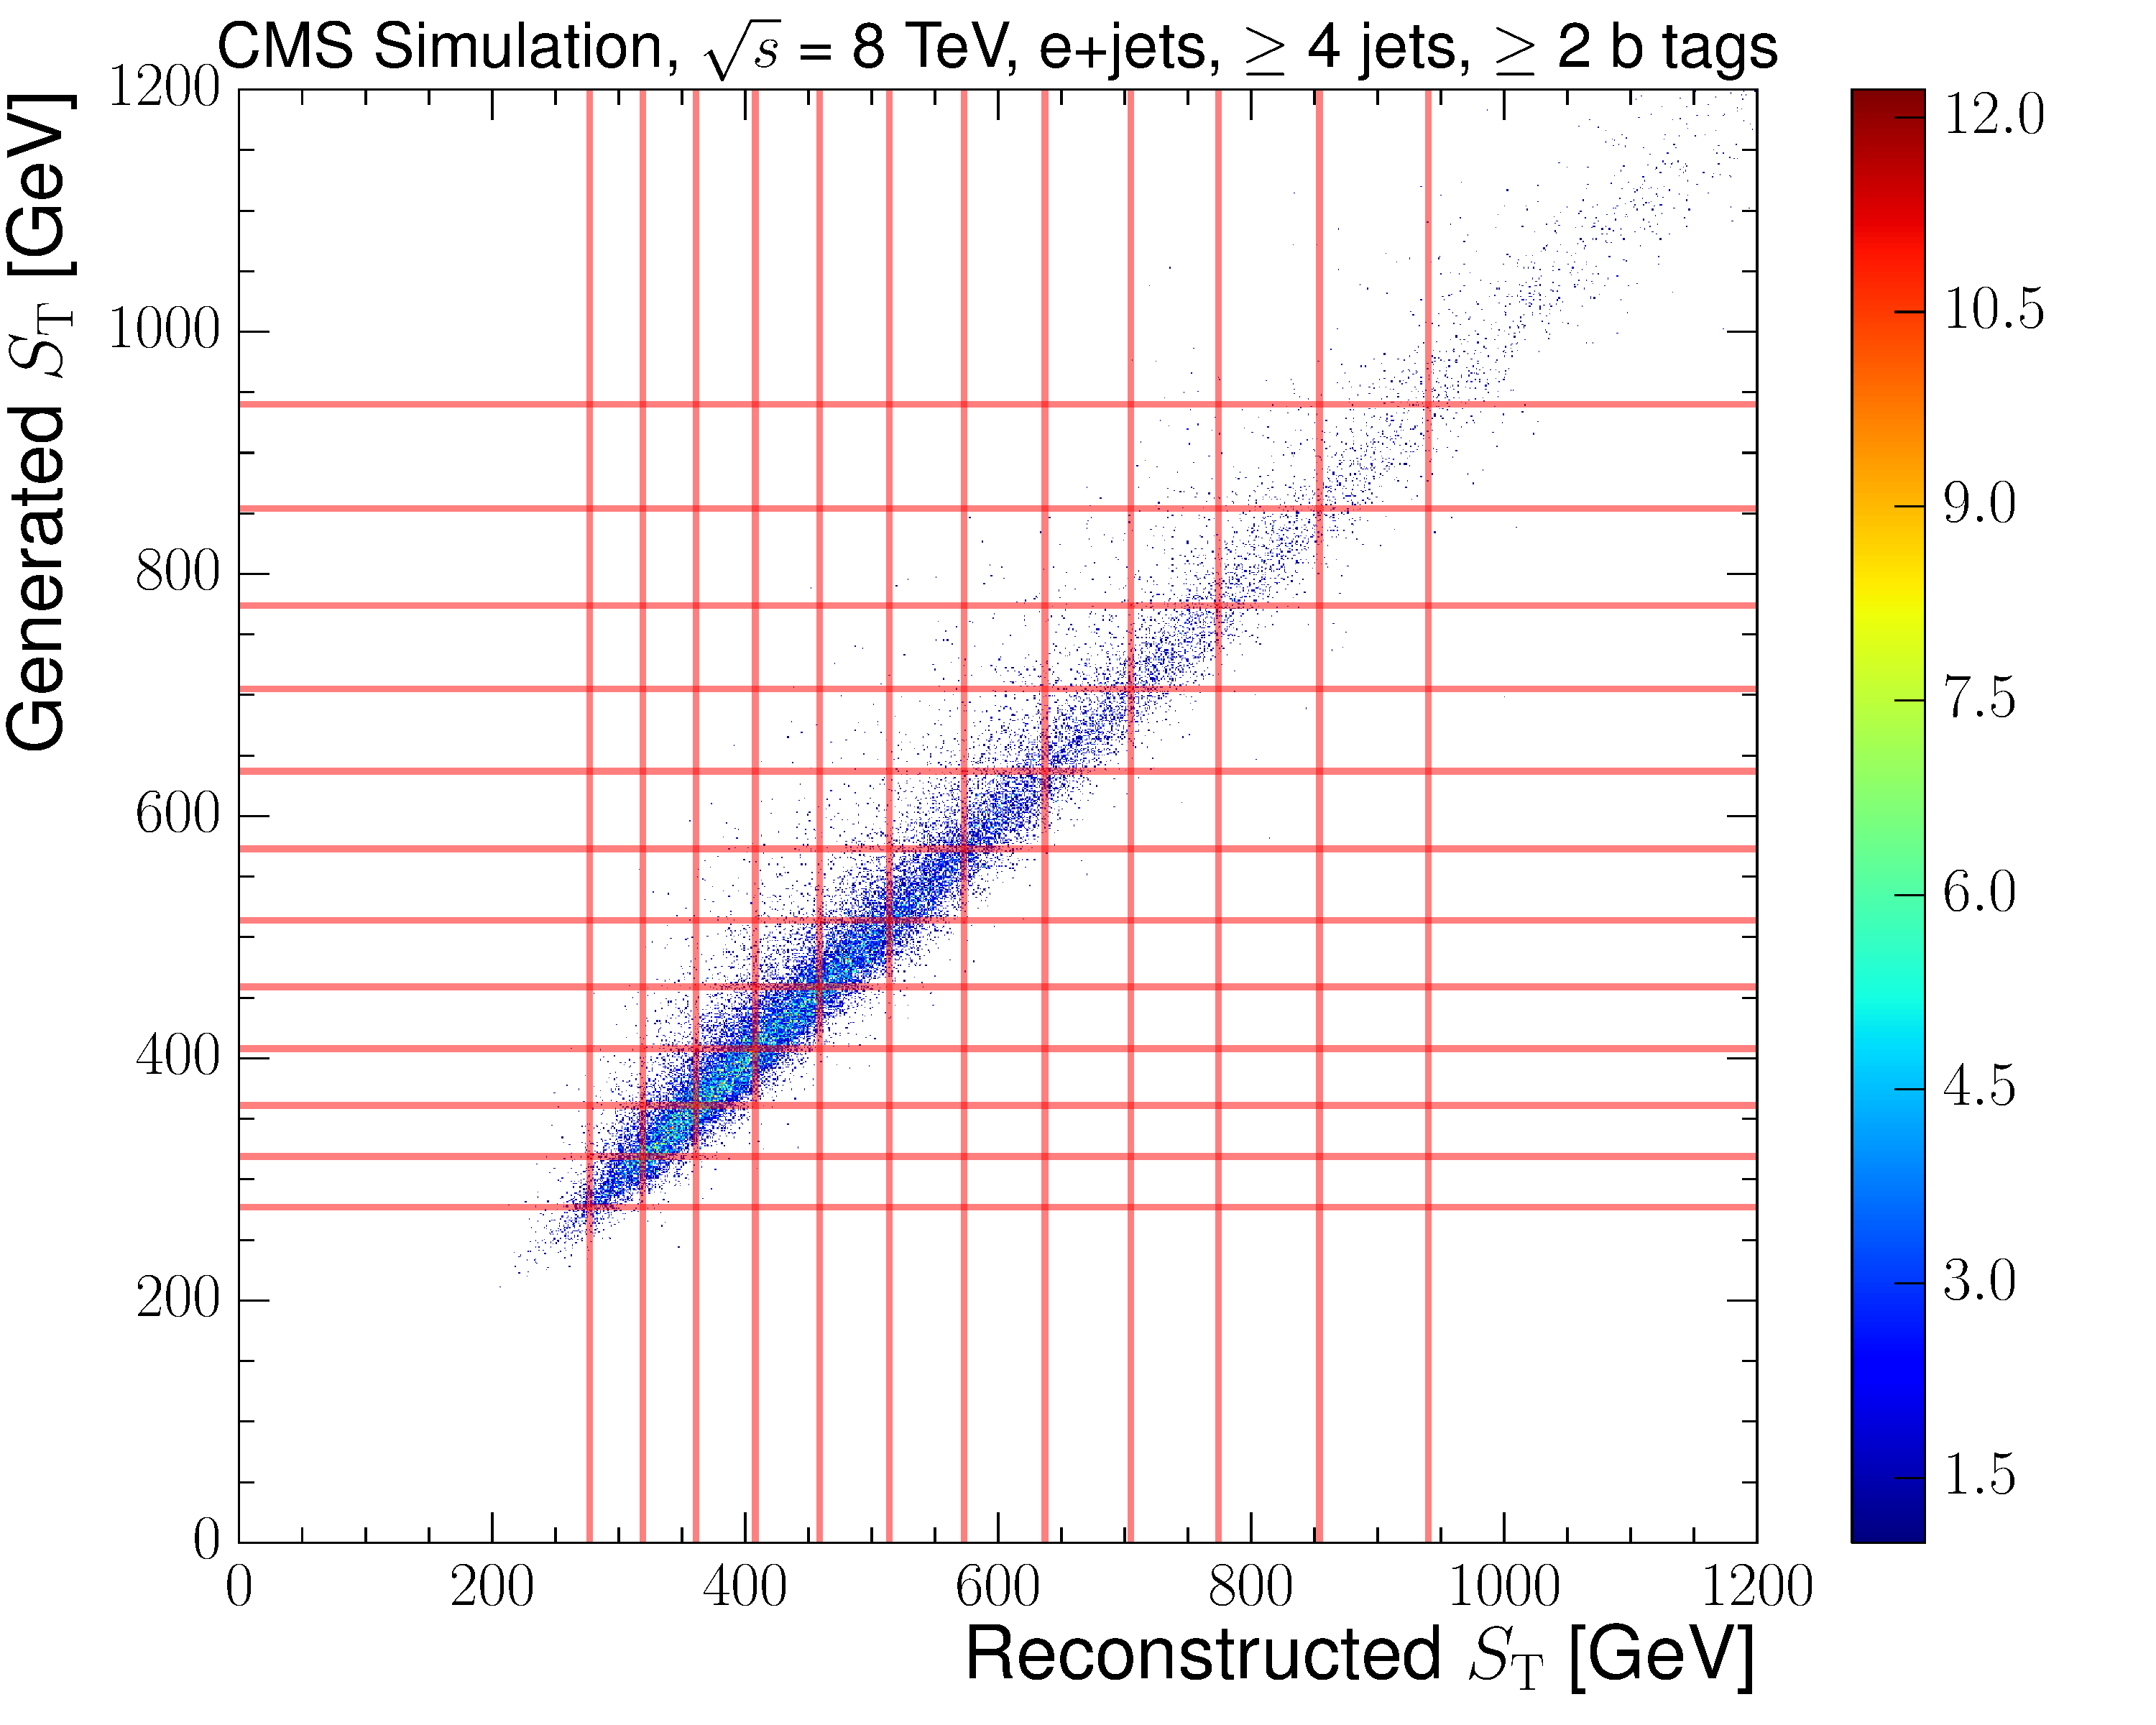
\includegraphics[width=0.48\textwidth]{Chapters/04_Analysis/04b_XSections/images/binning/electron_ST_8TeV.pdf}\hfill
     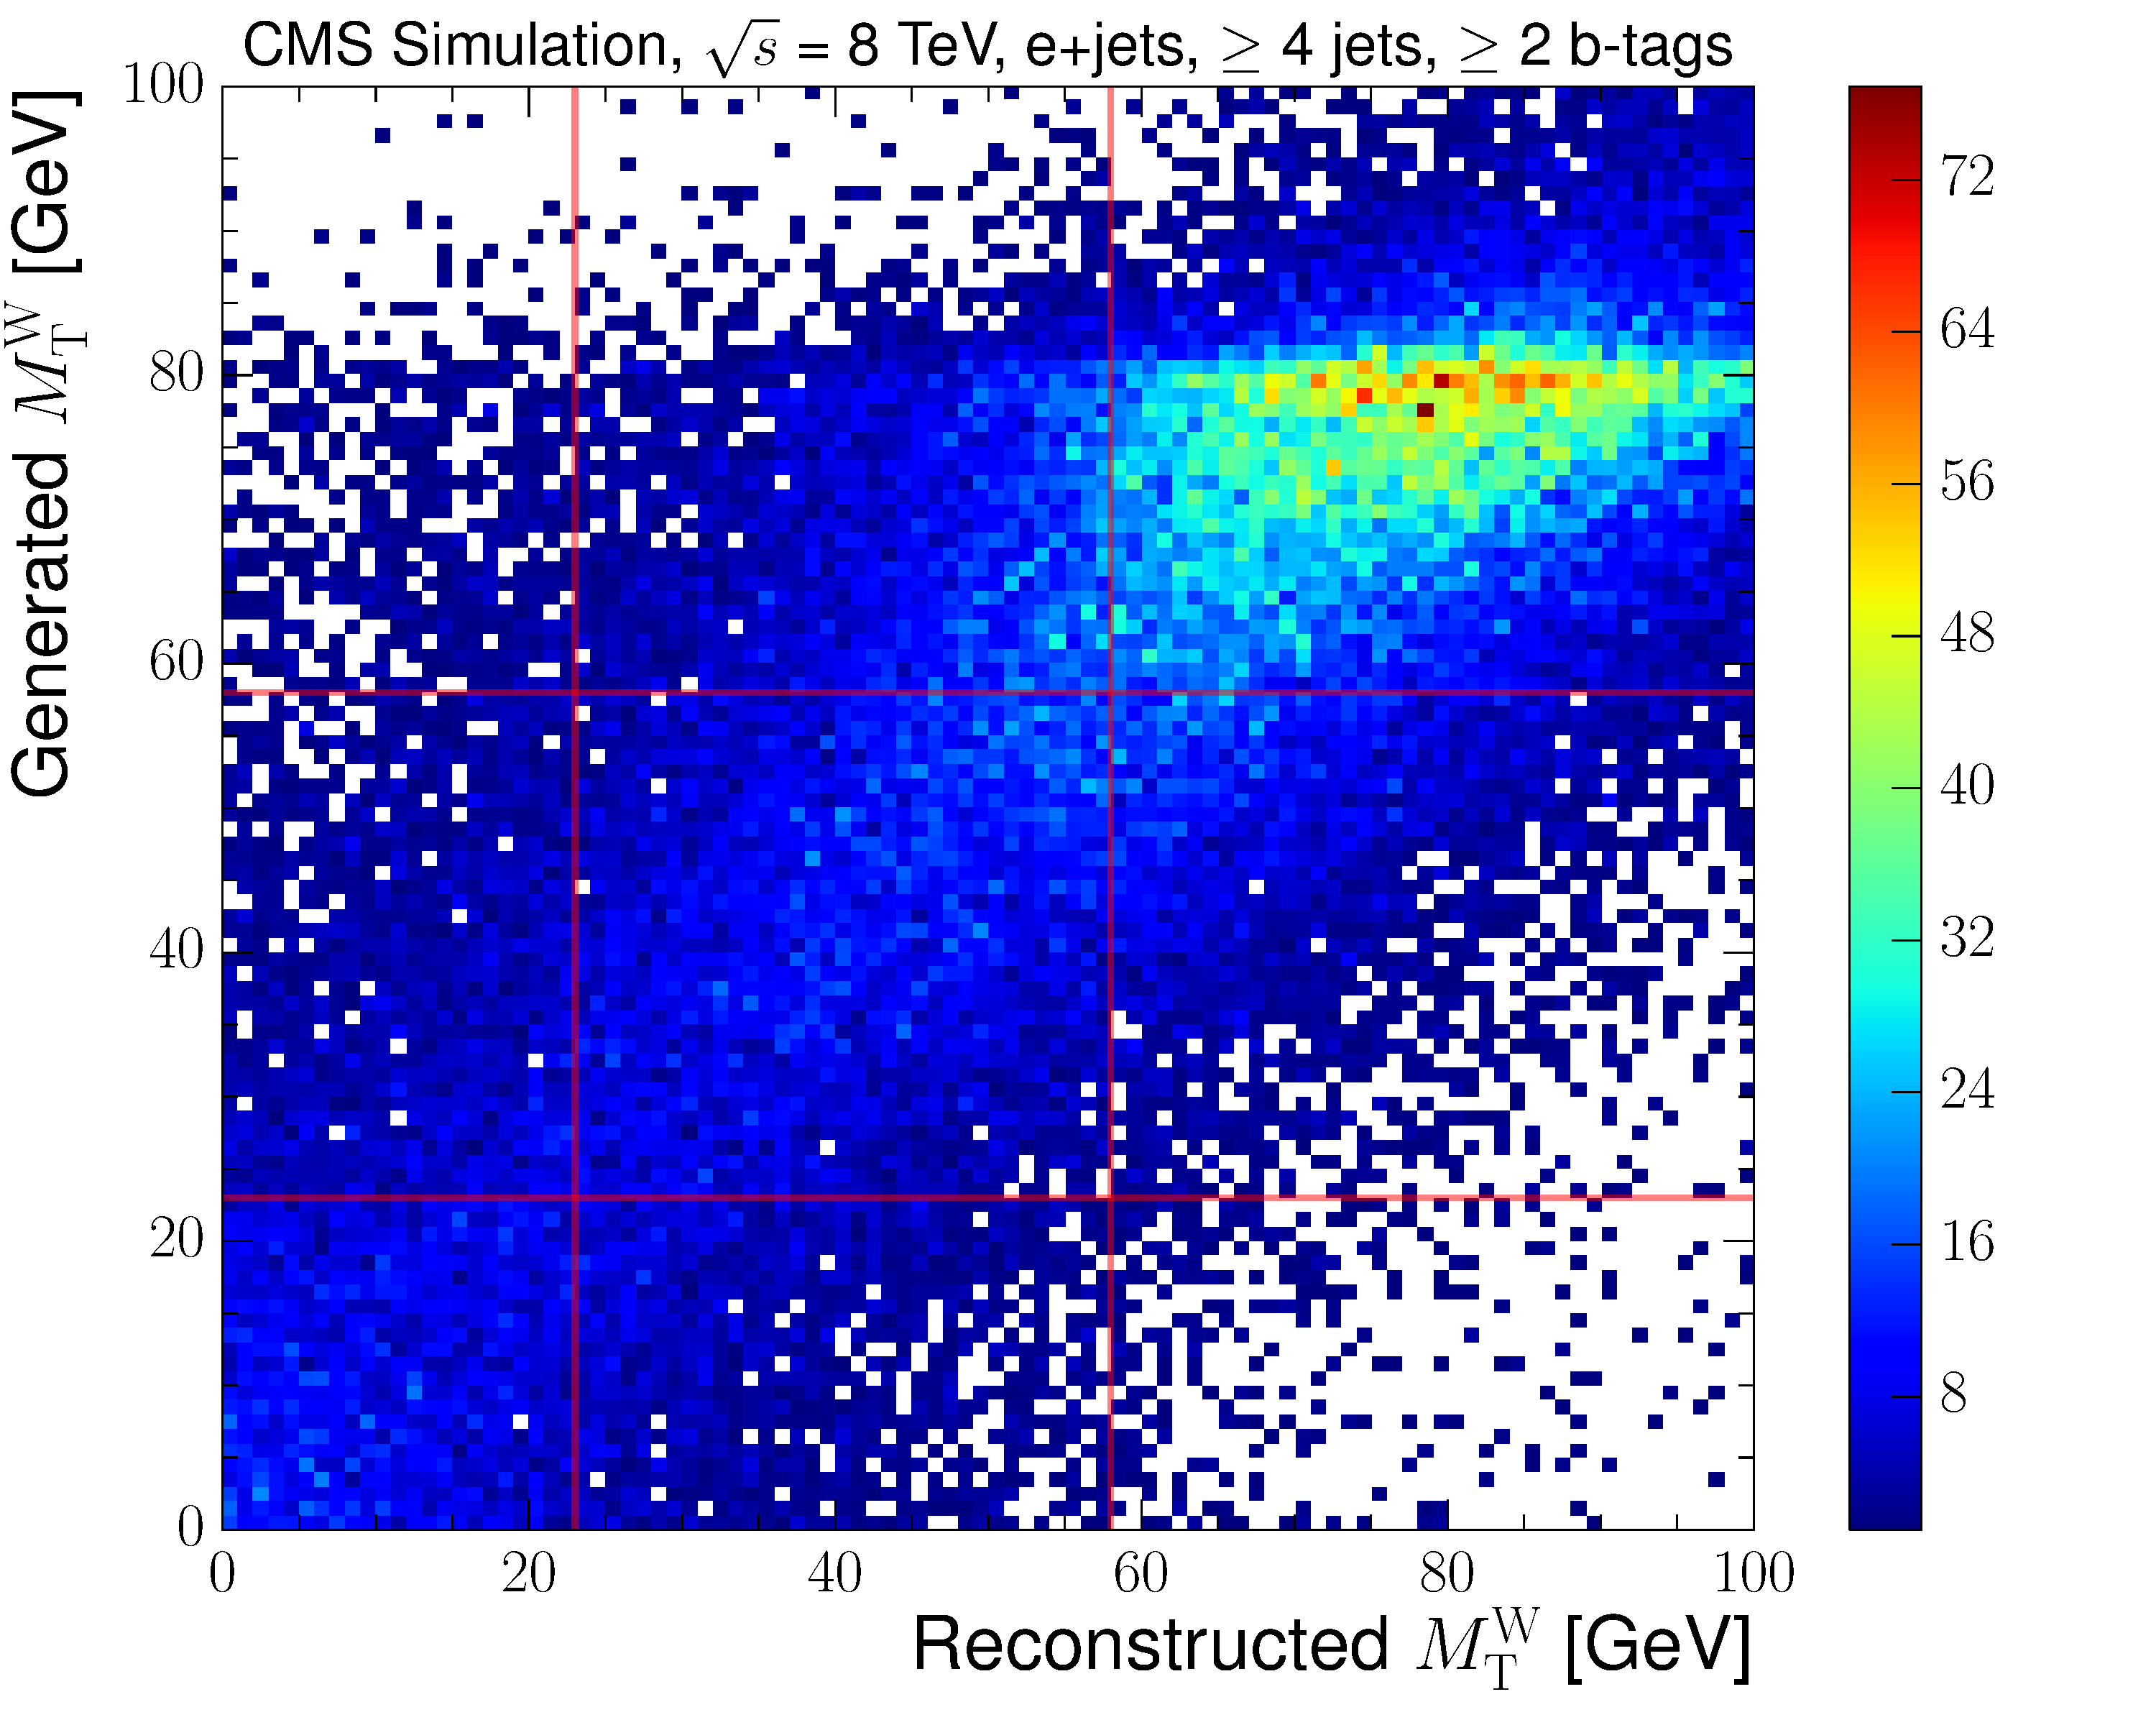
\includegraphics[width=0.48\textwidth]{Chapters/04_Analysis/04b_XSections/images/binning/electron_MT_8TeV.pdf}\\
	 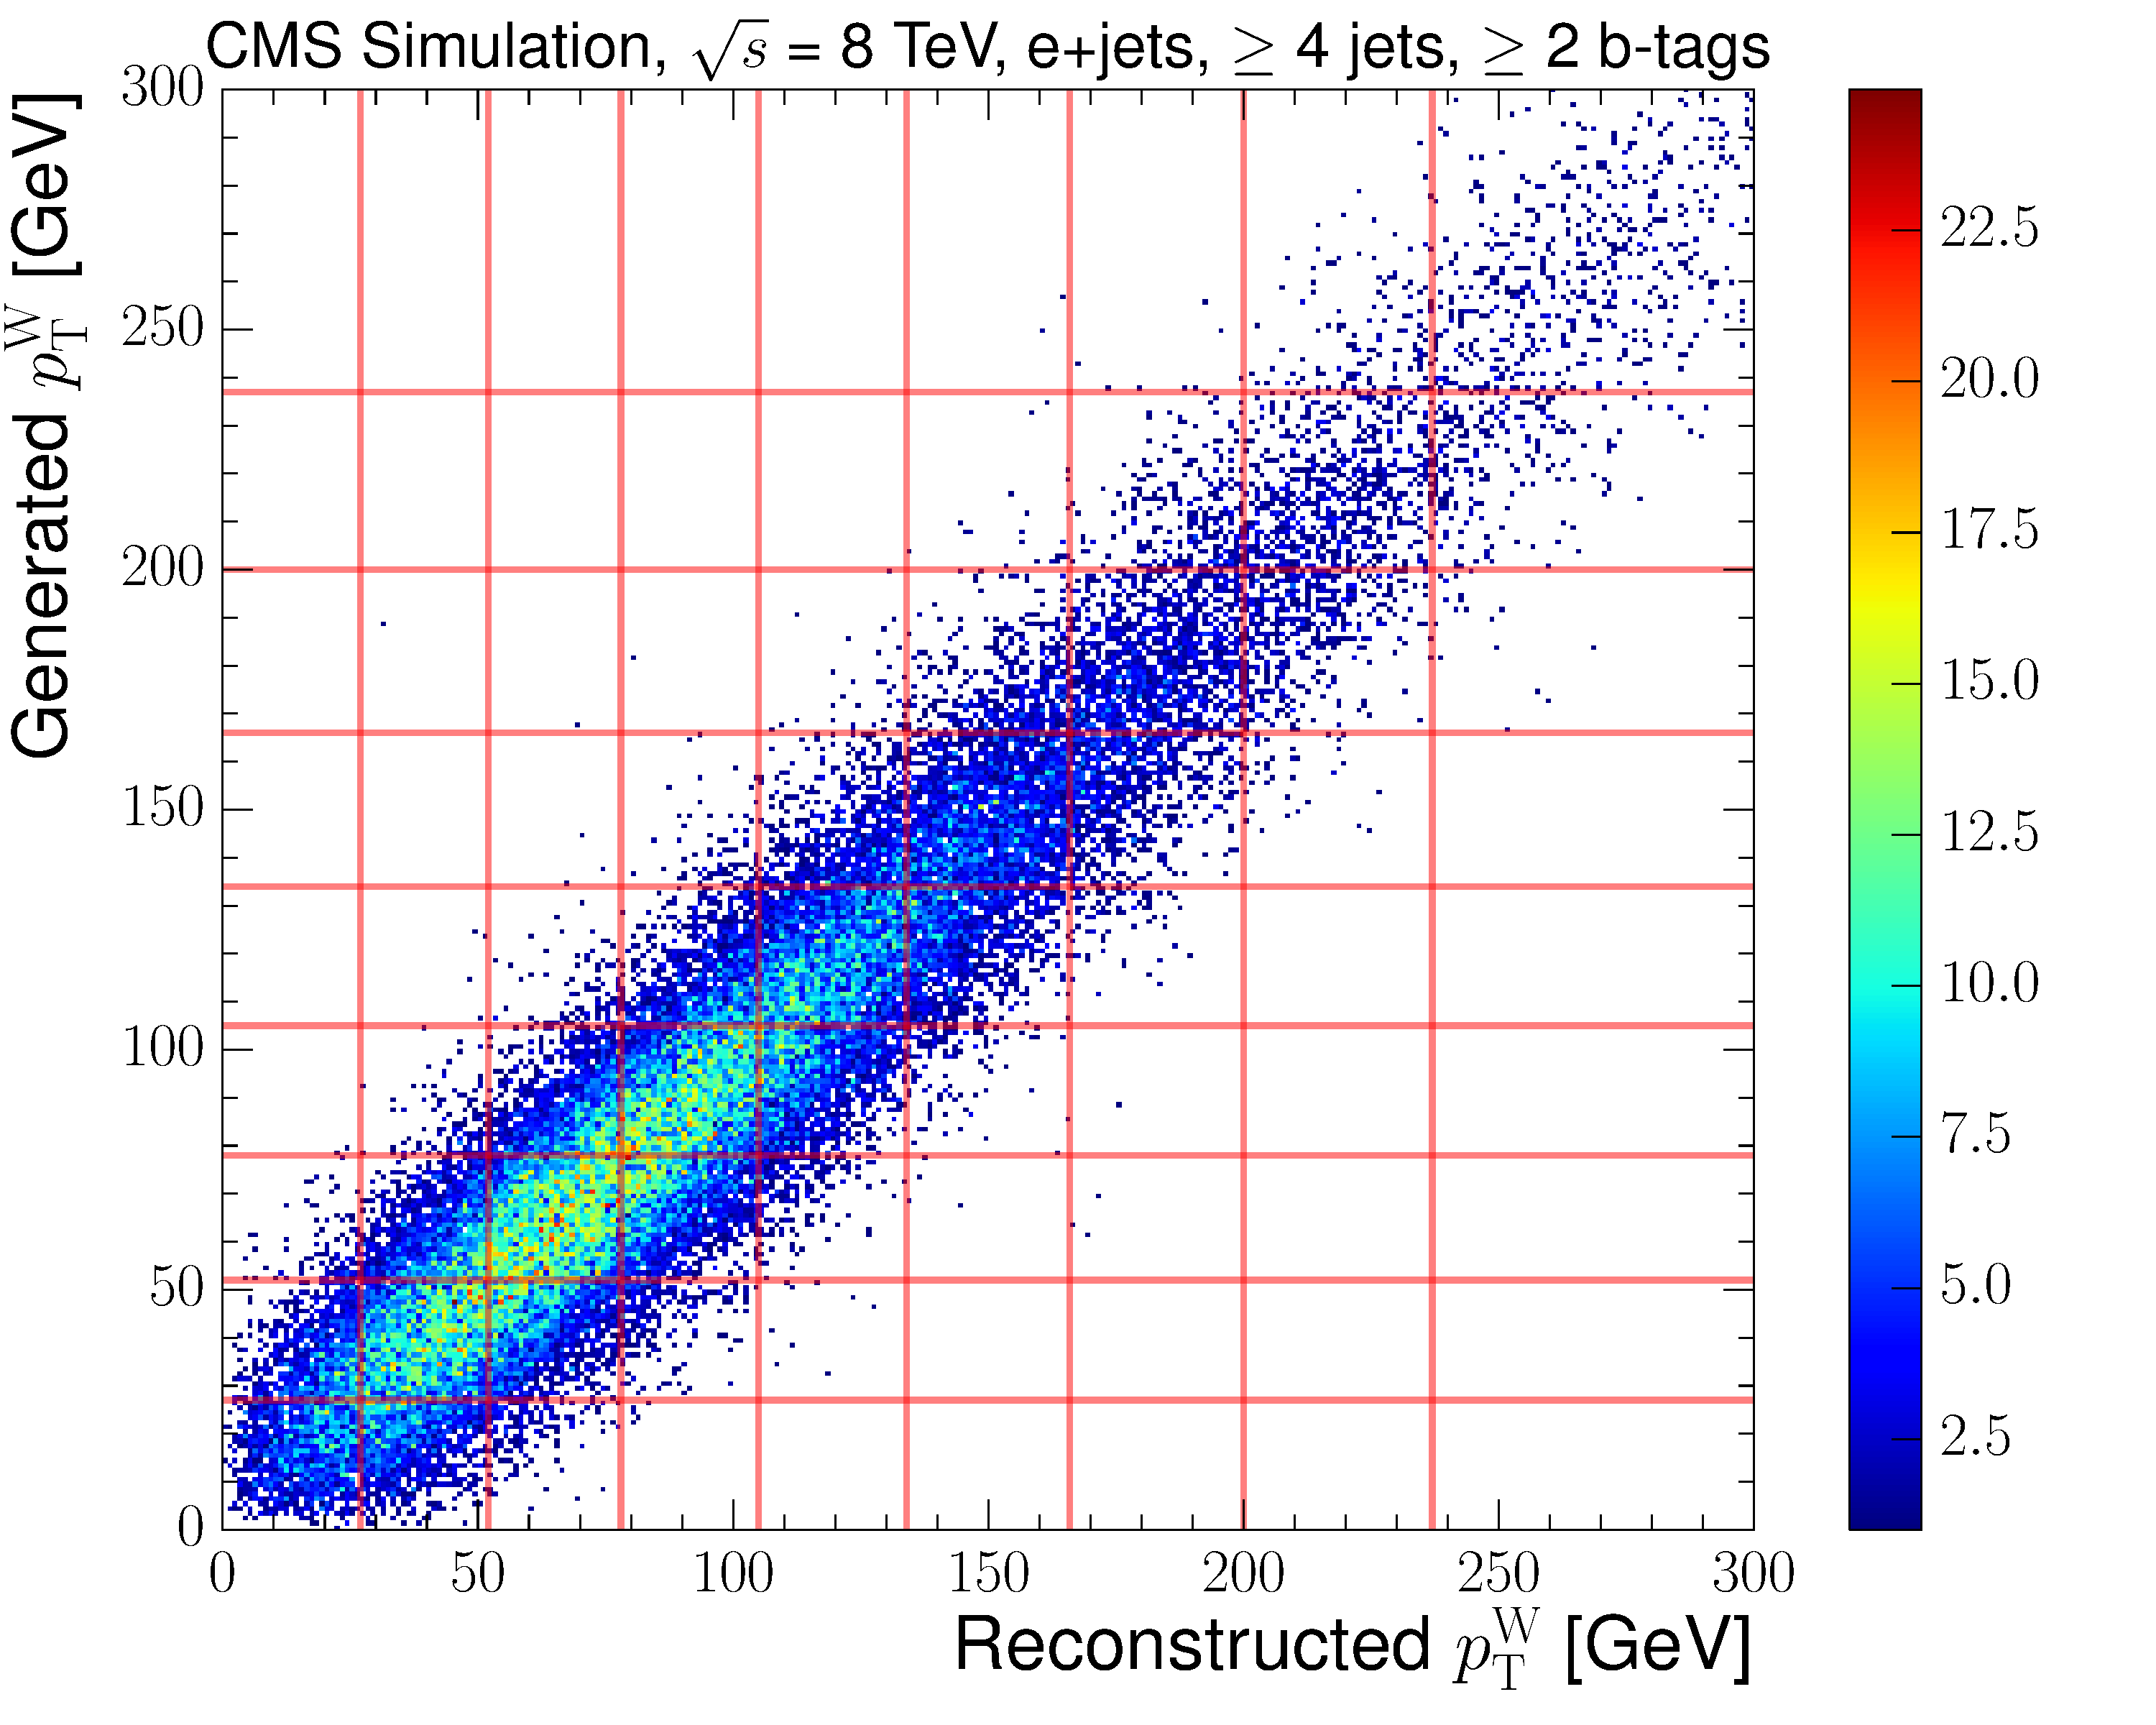
\includegraphics[width=0.48\textwidth]{Chapters/04_Analysis/04b_XSections/images/binning/electron_WPT_8TeV.pdf}\hfill
	 \caption{Generated versus reconstructed distributions of the primary variables \met (upper left), \HT (upper
	 right), \st (middle left), \mt (middle right) and \wpt (lower) with horizontal and vertical lines
	 representing the boundaries of the selected bins at $\sqrt{s}=8\TeV$ in the electron+ jets channel. These
	 distributions are obtained using \ttbar Monte Carlo simulation.}
     \label{fig:binning_8TeV_electron}
 \end{figure}
\FloatBarrier

\section{Maximum Likelihood Fit}
\label{maximum_likelihood_fit}
A maximum log likelihood fit of four templates to data in each bin of the primary variables is used to obtain
the number of events in each bin. The four templates used are \ttbar, single top, V+Jets (a combination of
W+Jets and Z+Jets events) and QCD. The template distributions are obtained from the following three
variables: the absolute pseudorapidity of the lepton (\abseta), the three-dimensional angle between the lepton
and the nearest \bjet ($\alpha$), and the invariant mass of the three jets with the highest \pt sum ($M3$).

The fit is carried out by maximising the log of the likelihood function (LL):

\begin{equation}
\label{log_likelihood}
LL\left(x_i, d_i\right) = -2 \log{\prod\limits_{i}\frac{x_i^{d_i}\cdot
e^{-x_i}}{d_i!}}=-2\sum\limits_{i}\log{\left(\frac{x_i^{d_i}\cdot e^{-x_i}}{d_i!}\right)}.
\end{equation}

where $i$ is the bin index in the template, $x_i$ is the total of all the templates in bin $i$, and $d_i$ is
the observed number of data events in  bin $i$. $x_i$ is defined to be

\begin{equation}
\label{eq:sum_mc}
x_i = \sum\limits_{j}N_{j}x_{i\,j},\;\text{with}\;\sum\limits_{i}\theta_{i\,j}=1\ for each process.
\end{equation}

where $\theta_{i\,j}$ represents the templates and $N_{j}$ represents the normalisations of the templates.
Fitting using more than one fitting variable (the three aforementioned fitting variables), the log likelihoods are summed:
\begin{equation}
\label{eq:log_L_final}
LL\left(x, d\right) = -\frac{2}{k} \sum\limits_{k} \log{L_k}
\end{equation}

where $L_k$ is the likelihood function of each of the different fit variables. Here the division by $k$
accounts for the fact that the same information is used in all three fit variables, and provides a
conservative estimate of the uncertainties in the resulting fitted parameters. The fit functions by adjusting
the normalisation of each template with the aim of equating $x_{i}$ and $d_{i}$ in each bin of each
template. The starting normalisations in the templates are obtained from simulation after the full selection
has been applied (this includes the QCD template, although the shape for this is obtained from data).

\subsection{Choice of templates}
\label{choice_of_templates}

Three fitting variables are used because no individual fit variable is able to distinguish between all four
templates used in the fit:

\begin{itemize}
  \item {\ttbar}
  \item{single-top}
  \item{V+jets (W+jets + Z+jets}
  \item{QCD multi-jet} 
\end{itemize}

\ttbar, single-top and V+jets templates are taken from simulation, while the QCD template is extracted from
data as described in Section~\ref{ss:background_selection}. The W+jets and Z+jets templates are combined
firstly due to the similar shapes of the distributions in these two background processes, and secondly due to
limited statistics available in simulation. The four template shapes in each of the three fitting variables
are shown in Figures~\ref{fig:fit_variable_distributions_7TeV} and \ref{fig:fit_variable_distributions_8TeV} for $\sqrt{s}=7\TeV$ and $\sqrt{s}=8\TeV$ respectively. This combination of fitting variables was selected because they are uncorrelated to the primary variables under
investigation, and they show good discrimination between the four templates.
Single top events have similar signatures to \ttbar events, with a central lepton from the decay of the single
top, leading to a single top template that is similar to the \ttbar template in the electron \abseta and muon
\abseta distributions. In the $\alpha$ distribution, the similarity is attributable to the fact that the
average boost for single top events is lower than in \ttbar events, leading to a wider single top template.
The M3 variable will be a combination of the jets from the hadronically decaying \tquark (a \bjet and two
other jets from the \W-boson) in \ttbar events, wheras in the other templates, M3 will simply correspond to
some random combination of jets in the event. Hence, M3 shows the best discrimination between the single top
and \ttbar templates.

\begin{figure}[hbtp]
    \centering
     \includegraphics[width=0.48\textwidth]{Chapters/04_Analysis/04b_XSections/images/7TeV/fit_variables/MET/electron_absolute_eta/MET_inclusive_electron_absolute_eta_2orMoreBtags_templates.pdf}\hfill
     
\includegraphics[width=0.48\textwidth]{Chapters/04_Analysis/04b_XSections/images/placeholder.png}\\
     %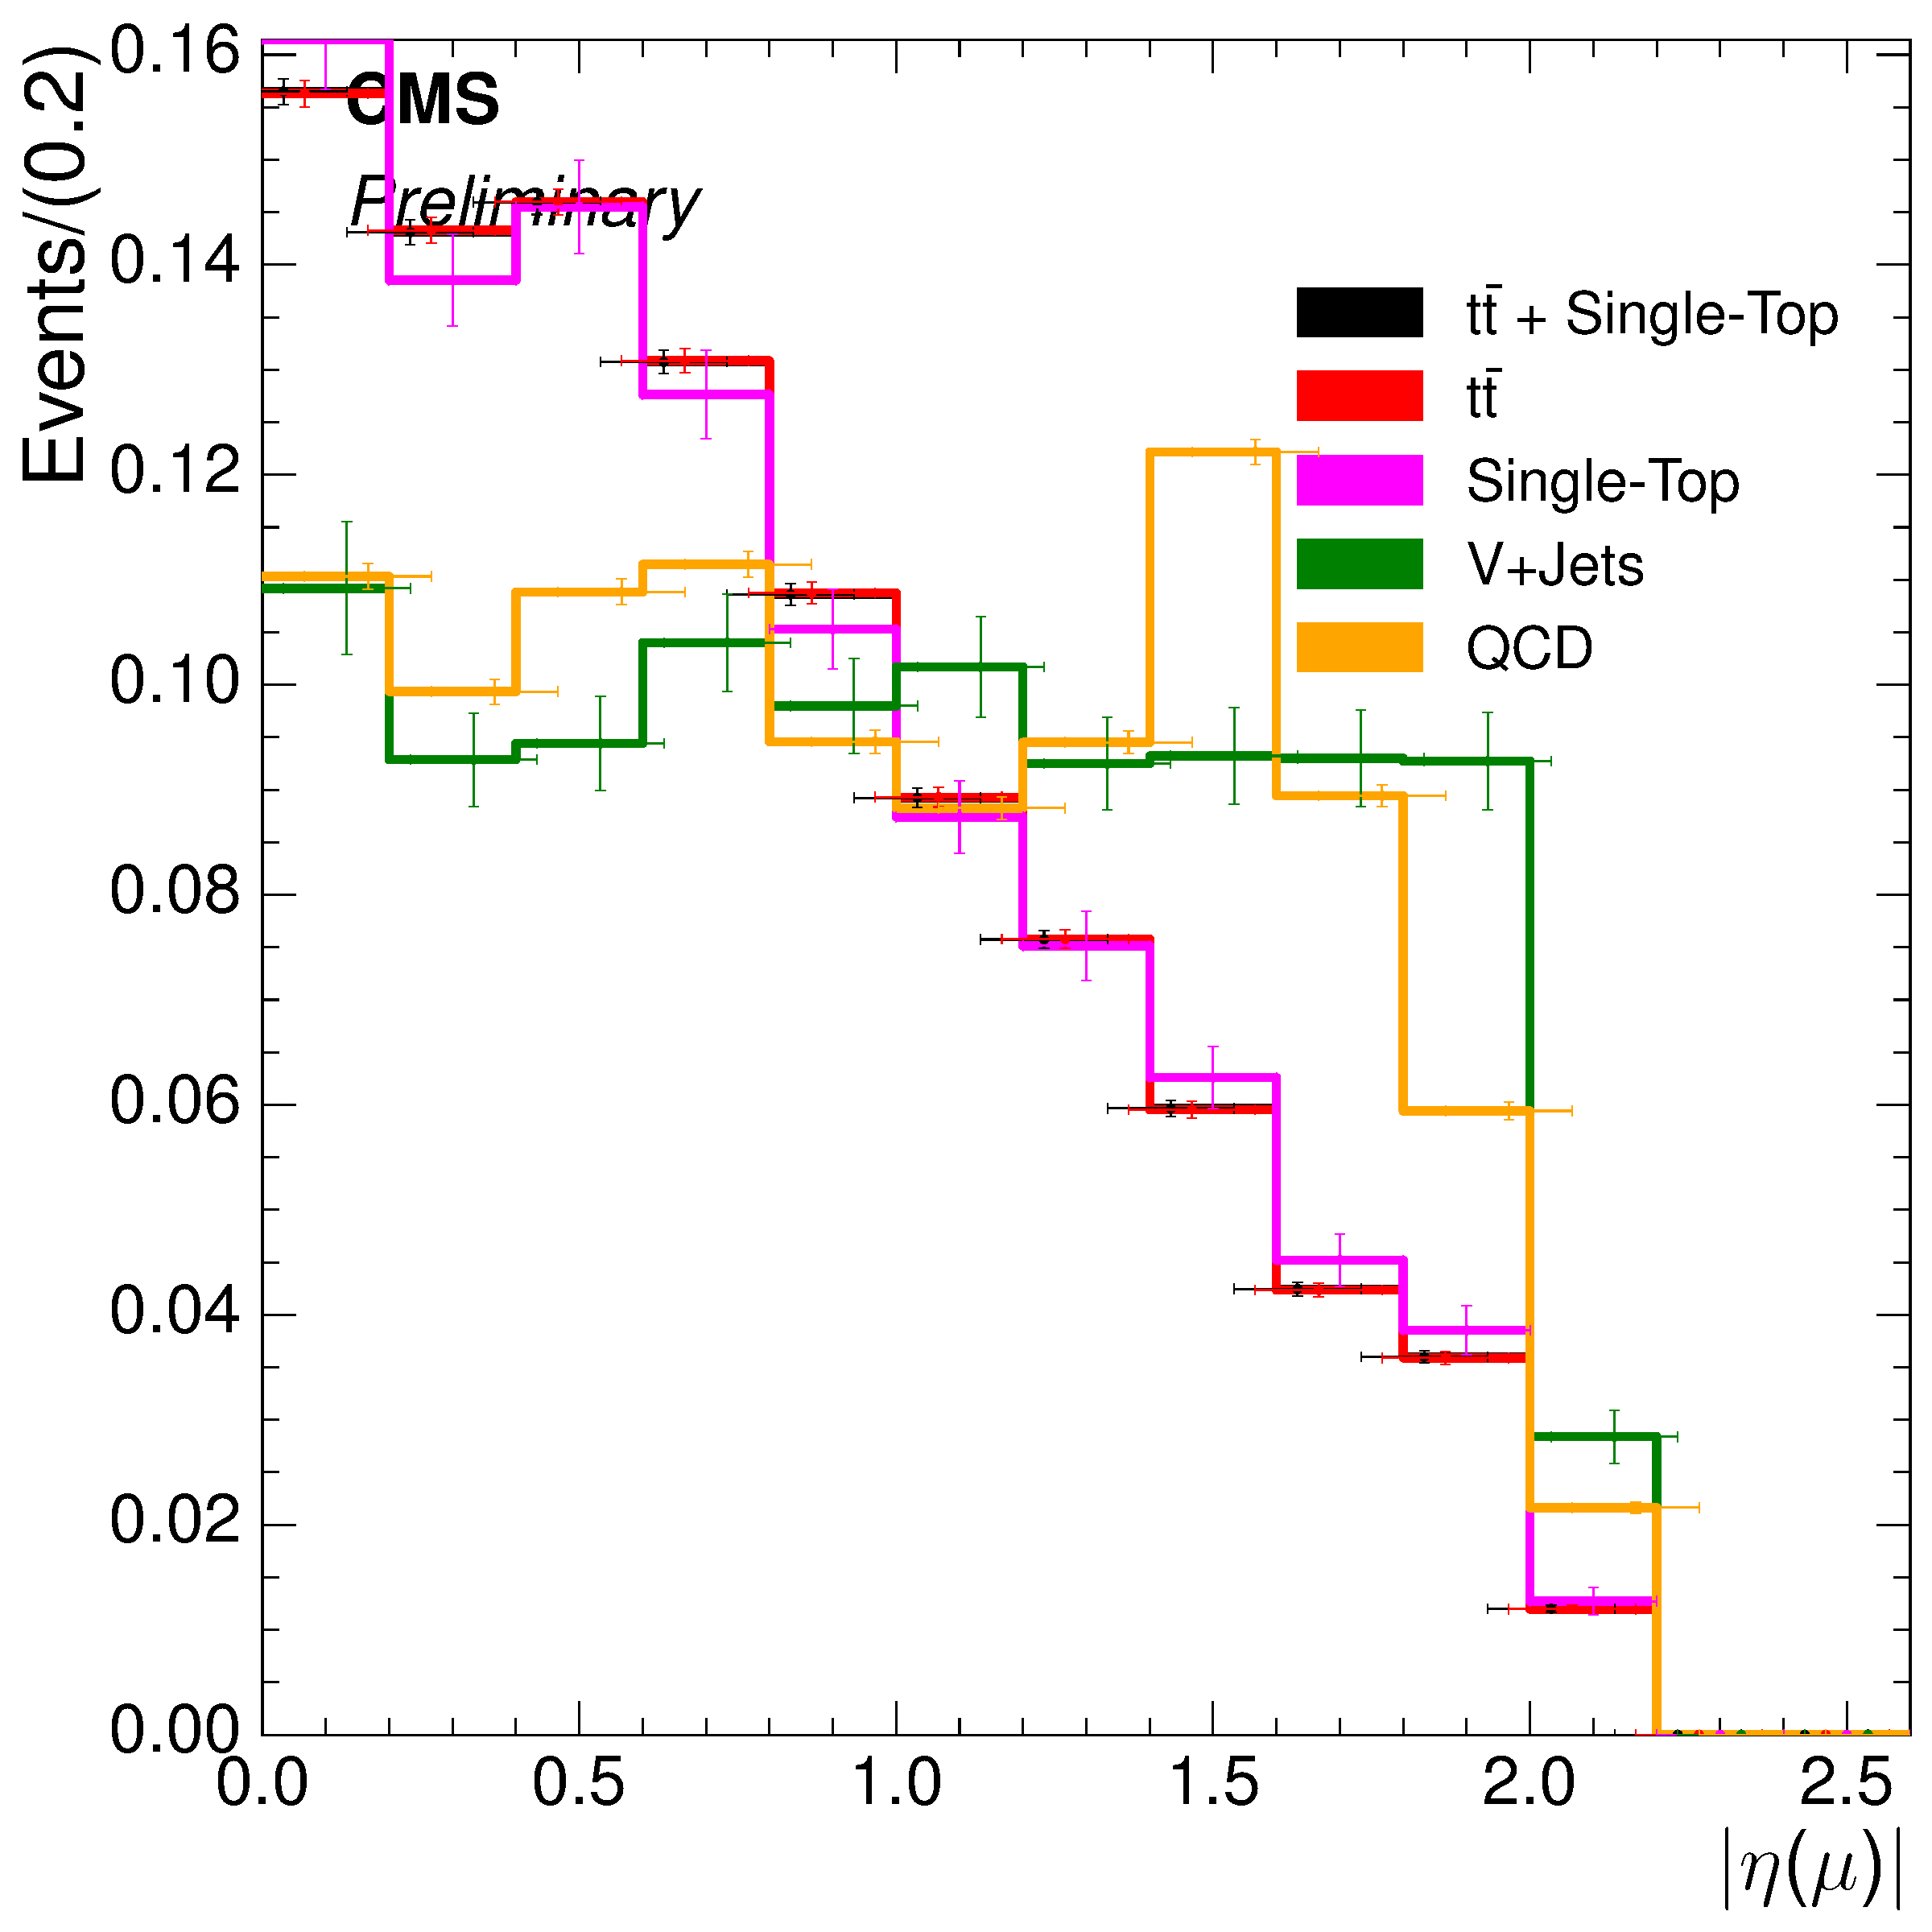
\includegraphics[width=0.48\textwidth]{Chapters/04_Analysis/04b_XSections/images/7TeV/fit_variables/MET/muon_absolute_eta/MET_inclusive_muon_absolute_eta_2orMoreBtags_templates.pdf}\\    
     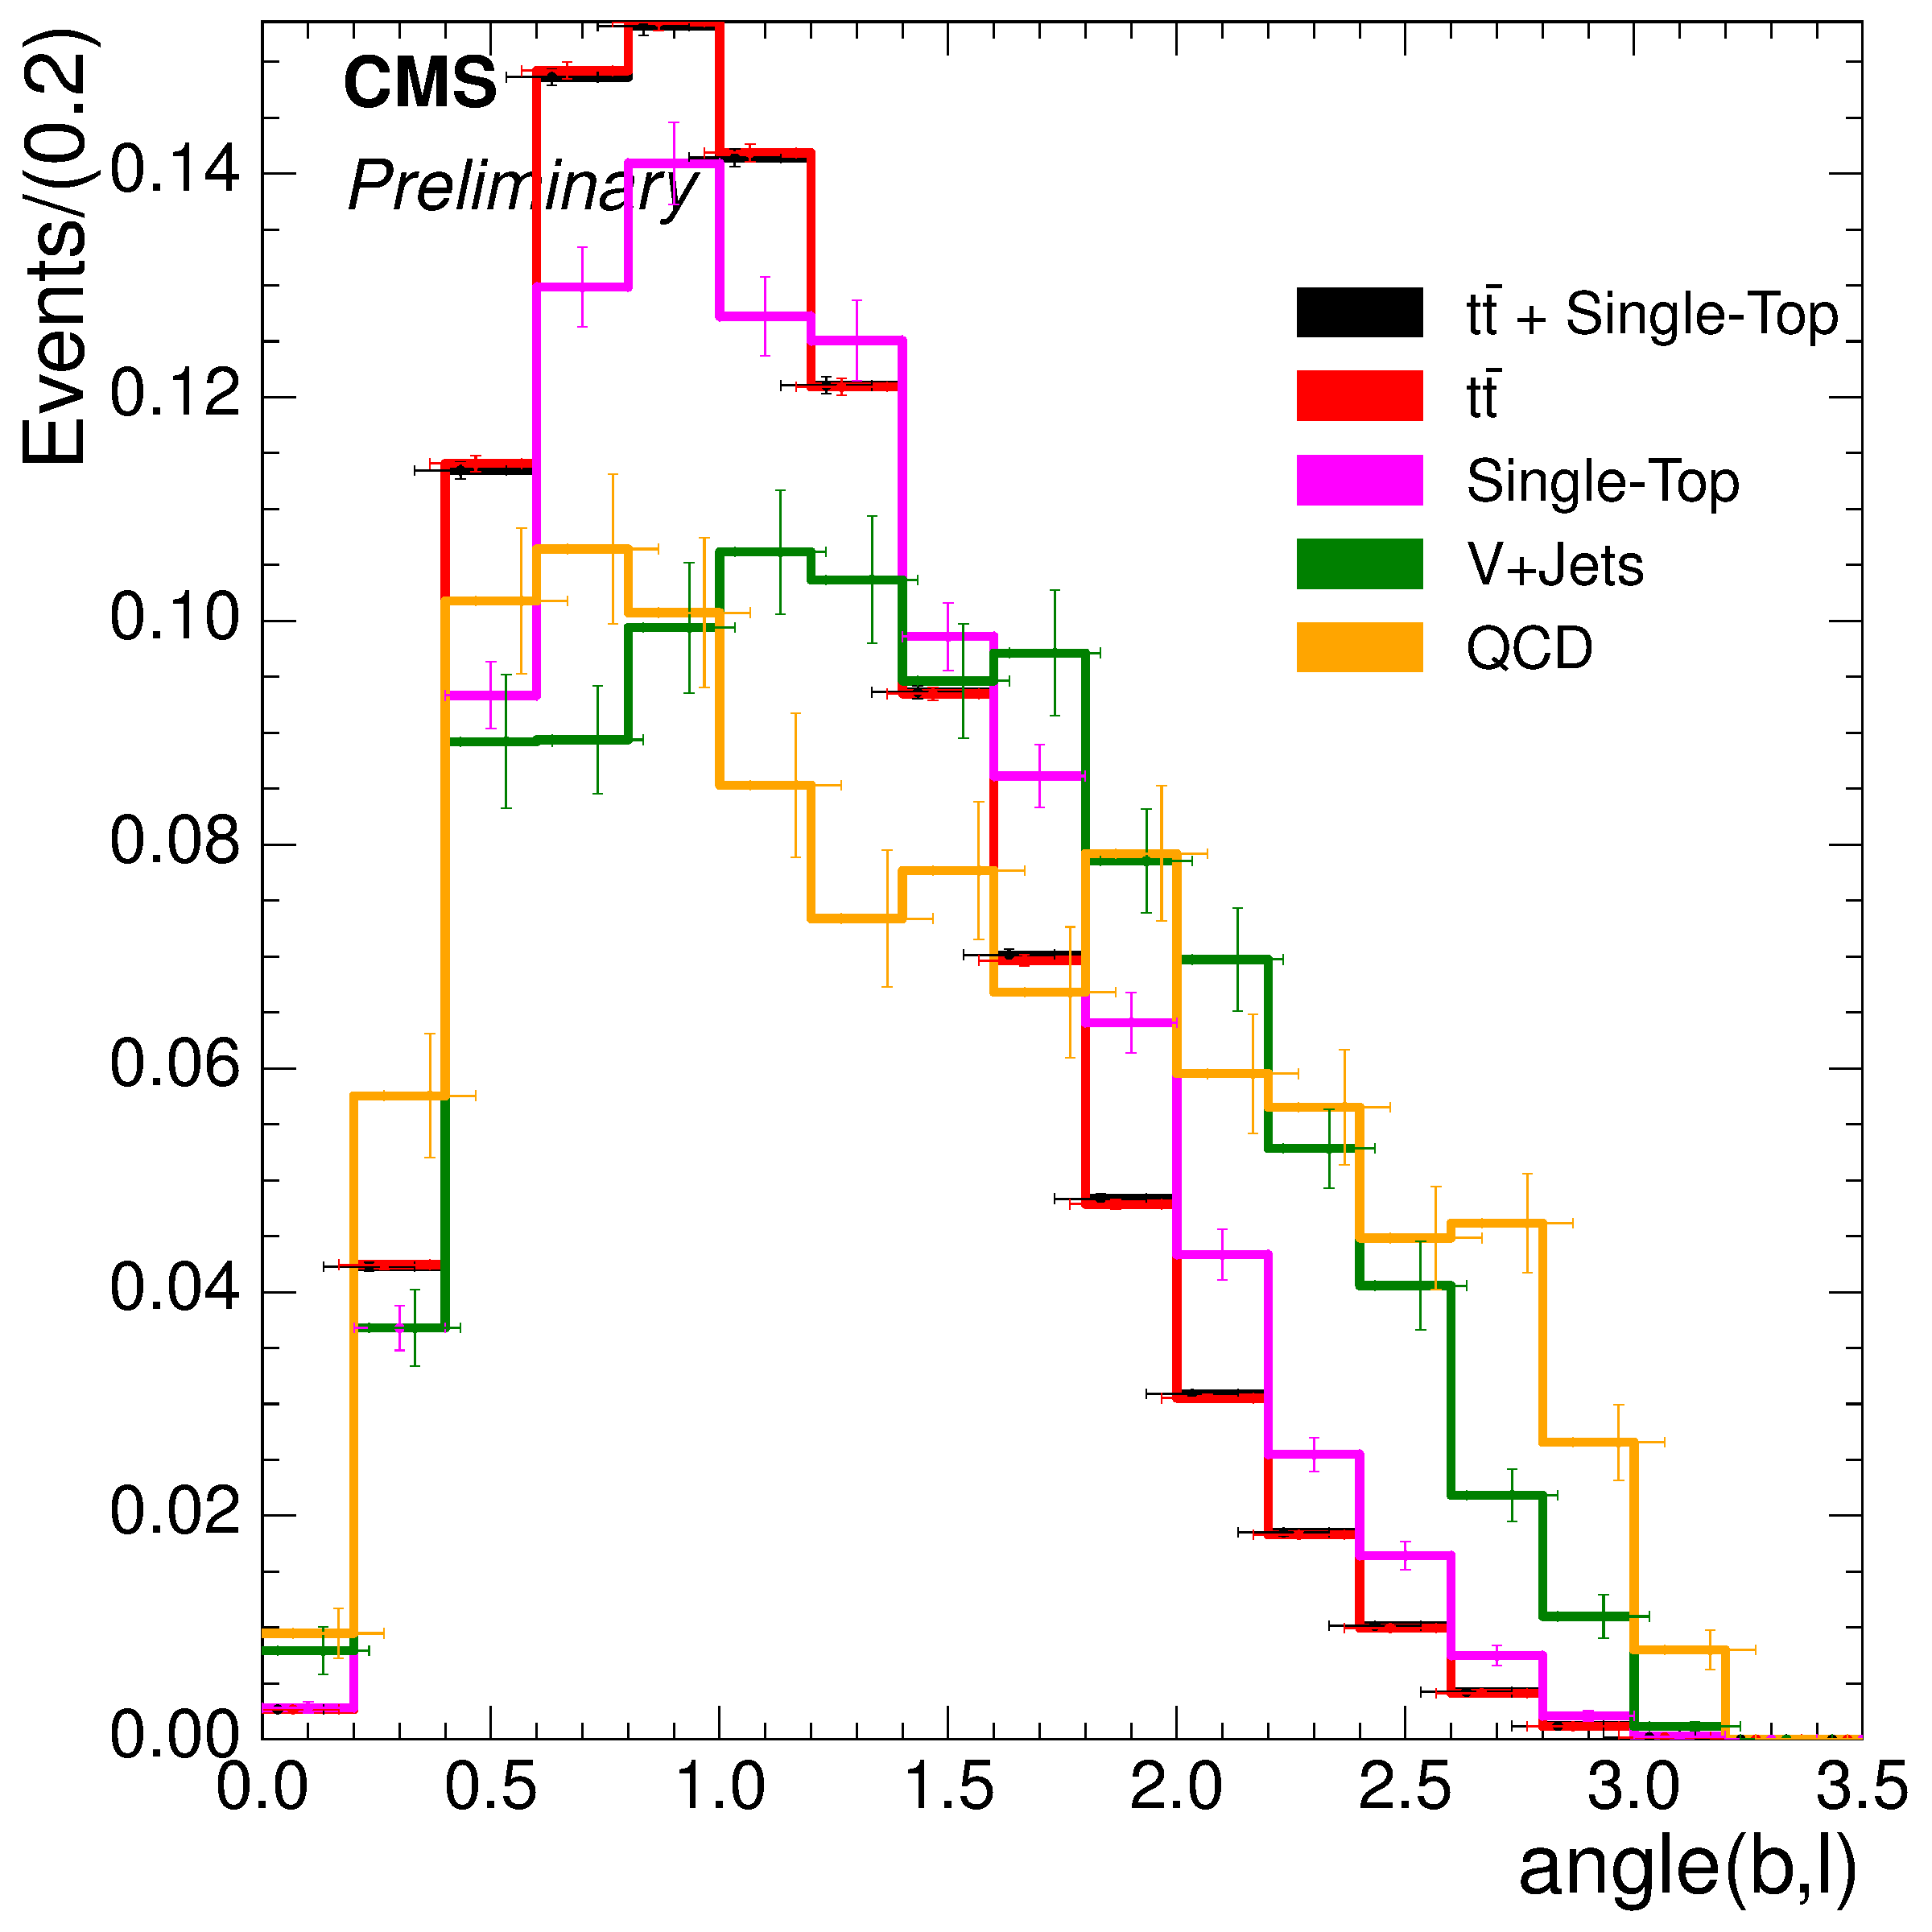
\includegraphics[width=0.48\textwidth]{Chapters/04_Analysis/04b_XSections/images/7TeV/fit_variables/MET/angle_bl/MET_inclusive_angle_bl_2orMoreBtags_templates.pdf}\hfill
     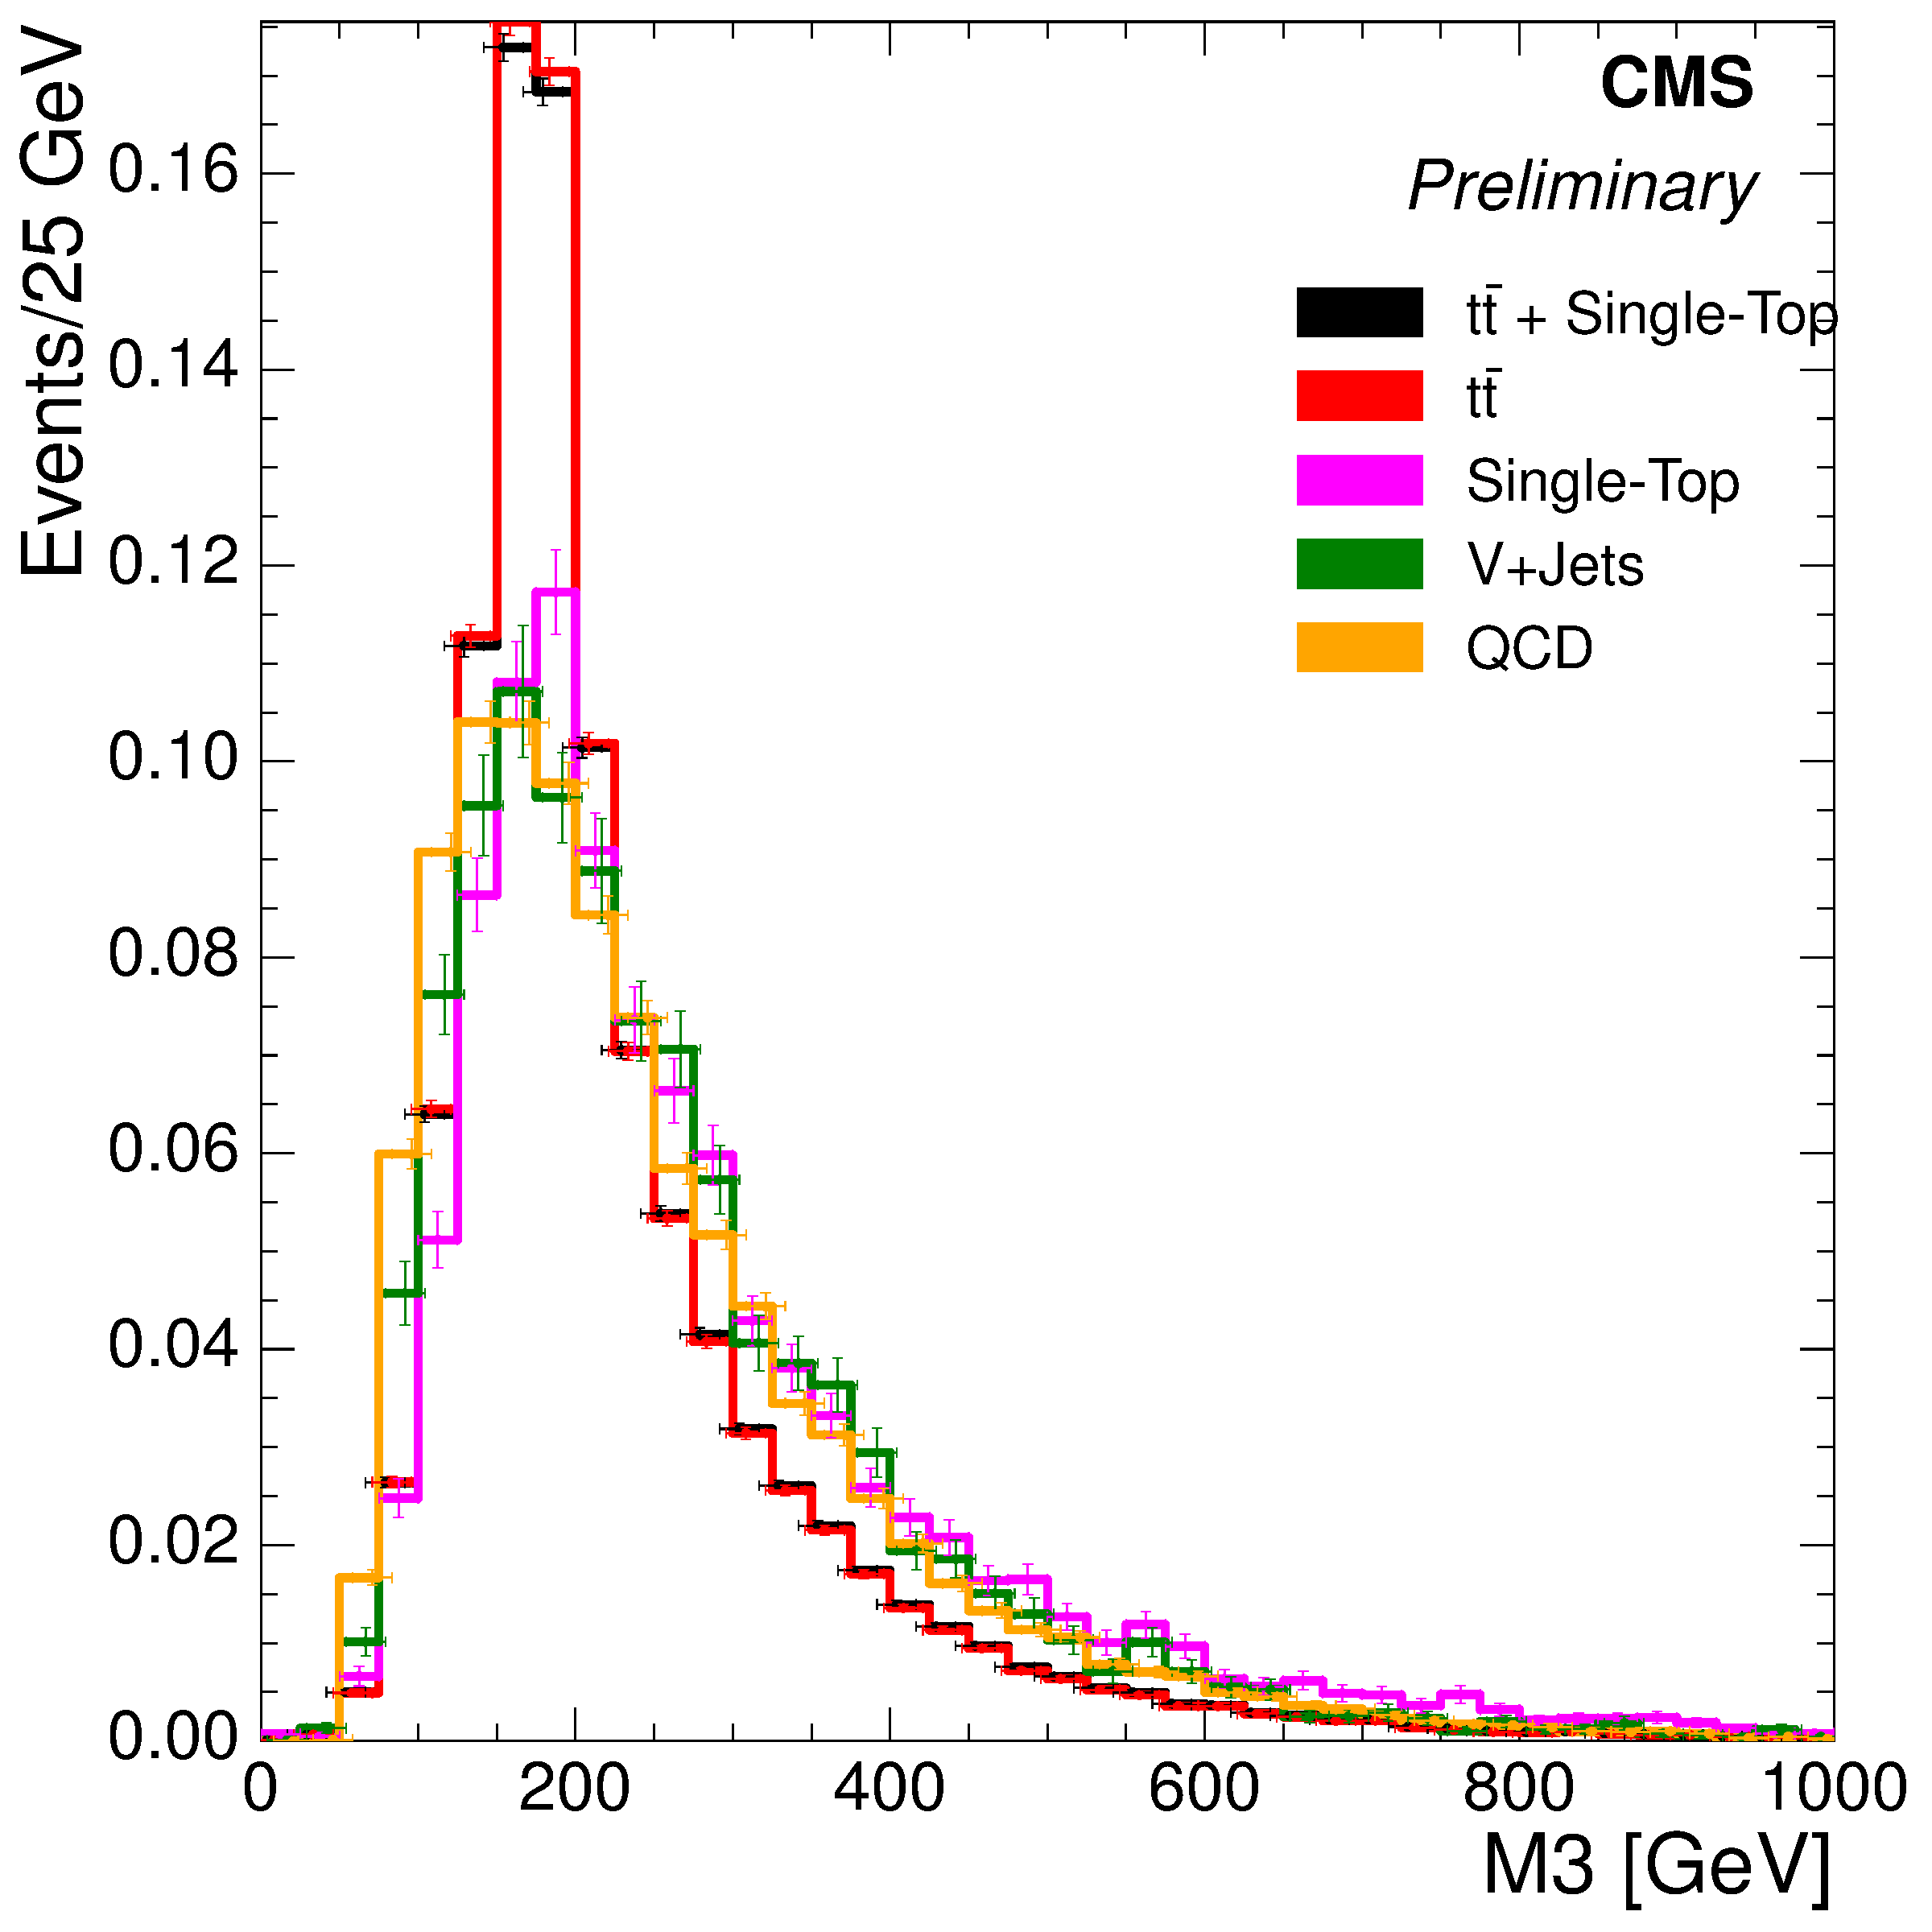
\includegraphics[width=0.48\textwidth]{Chapters/04_Analysis/04b_XSections/images/7TeV/fit_variables/MET/M3/MET_inclusive_M3_2orMoreBtags_templates.pdf}\\
	 \caption{Normalised distributions of the four templates for the three fit variables at $\sqrt{s}=7\TeV$,
	 inclusive across all primary variable bins: electron \abseta (upper left), muon \abseta (upper right),
	 $\alpha$ (lower left) and M3 (lower right).}
     \label{fig:fit_variable_distributions_7TeV}
\end{figure}

\begin{figure}[hbtp]
    \centering
     \includegraphics[width=0.48\textwidth]{Chapters/04_Analysis/04b_XSections/images/8TeV/fit_variables/MET/electron_absolute_eta/MET_inclusive_electron_absolute_eta_2orMoreBtags_templates.pdf}\hfill
     
\includegraphics[width=0.48\textwidth]{Chapters/04_Analysis/04b_XSections/images/placeholder.png}\hfill
     %\includegraphics[width=0.48\textwidth]{Chapters/04_Analysis/04b_XSections/images/7TeV/fit_variables/MET/muon_absolute_eta/MET_inclusive_muon_absolute_eta_2orMoreBtags_templates.pdf}\\    
     \includegraphics[width=0.48\textwidth]{Chapters/04_Analysis/04b_XSections/images/8TeV/fit_variables/MET/angle_bl/MET_inclusive_angle_bl_2orMoreBtags_templates.pdf}\hfill
     \includegraphics[width=0.48\textwidth]{Chapters/04_Analysis/04b_XSections/images/8TeV/fit_variables/MET/M3/MET_inclusive_M3_2orMoreBtags_templates.pdf}\\
	 \caption{Normalised distributions of the four templates for the three fit variables at $\sqrt{s}=8\TeV$,
	 inclusive across all primary variable bins: electron \abseta (upper left), muon \abseta (upper right),
	 $\alpha$ (lower left) and M3 (lower right).}
     \label{fig:fit_variable_distributions_8TeV}
\end{figure}
\FloatBarrier

The QCD templates inclusive across all bins of the primary variables are used because of low statistics
in the QCD background selection in higher bins. Figure~\ref{fig:fit_variable_qcd_comparisons_8TeV} shows a
comparison between QCD templates at $\sqrt{s}=8\TeV$ in the lowest three bins of the \met variable and also
the inclusive \met QCD template. It can be seen that the third \met bin already shows low numbers of events,
meaning the inclusive template is largely shaped by events in the first two bins. Therefore, the inclusive QCD
template is used rather than those in individual bins. Similar plots showing the same behaviour for the other
primary variables are shown in Appendix~\ref{as:fitting_variable_QCD_template_comparisons}.

\begin{figure}[hbtp]
    \centering
     \includegraphics[width=0.48\textwidth]{Chapters/04_Analysis/04b_XSections/images/8TeV/fit_variables/MET/electron_absolute_eta/qcd/MET_electron_absolute_eta_0orMoreBtag_QCD_template_comparison.pdf}\hfill
     \includegraphics[width=0.48\textwidth]{Chapters/04_Analysis/04b_XSections/images/placeholder.png}\hfill
     %\includegraphics[width=0.48\textwidth]{Chapters/04_Analysis/04b_XSections/images/7TeV/fit_variables/MET/muon_absolute_eta/qcd/MET_inclusive_muon_absolute_eta_2orMoreBtags_templates.pdf}\\    
     \includegraphics[width=0.48\textwidth]{Chapters/04_Analysis/04b_XSections/images/8TeV/fit_variables/MET/angle_bl/qcd/MET_angle_bl_1orMoreBtag_QCD_template_comparison.pdf}\hfill
     \includegraphics[width=0.48\textwidth]{Chapters/04_Analysis/04b_XSections/images/8TeV/fit_variables/MET/M3/qcd/MET_M3_0orMoreBtag_QCD_template_comparison.pdf}\\
	 \caption{Normalised distributions of the QCD templates for the three fit variables at $\sqrt{s}=8\TeV$
	 inclusive across all \met bins and for the lowest three \met bins: electron \abseta (upper
	 left), muon \abseta (upper right), $\alpha$ (lower left) and M3 (lower right).}
     \label{fig:fit_variable_qcd_comparisons_8TeV}
\end{figure}

An inclusive template is also used in the V+jets (W+jets + Z+jets template) for the same reason.
Figure~\ref{fig:MET_fit_variable_vjets_comparisons_8TeV} shows a comparison between the V+jets templates at
$\sqrt{s}=8\TeV$ in each \met bin and also the inclusive \met V+jets template.
As is the case for the QCD background template, it can be seen in the V+jets templates that there are
diminished statistics available in higher bins, and the inclusive template shape is largely governed by the
lower bins. Similar plots demonstrating the same behaviour for the other primary variables are shown in
Appendix~\ref{as:fitting_variable_vjets_template_comparisons}.

\begin{figure}[hbtp]
    \centering
     \includegraphics[width=0.48\textwidth]{Chapters/04_Analysis/04b_XSections/images/8TeV/fit_variables/MET/electron_absolute_eta/vjets/MET_electron_absolute_eta_2orMoreBtags_VJets_template_comparison.pdf}\hfill
     \includegraphics[width=0.48\textwidth]{Chapters/04_Analysis/04b_XSections/images/placeholder.png}\\
     %\includegraphics[width=0.48\textwidth]{Chapters/04_Analysis/04b_XSections/images/7TeV/fit_variables/MET/muon_absolute_eta/vjets/MET_inclusive_muon_absolute_eta_2orMoreBtags_templates.pdf}\\    
     \includegraphics[width=0.48\textwidth]{Chapters/04_Analysis/04b_XSections/images/8TeV/fit_variables/MET/angle_bl/vjets/MET_angle_bl_2orMoreBtags_VJets_template_comparison.pdf}\hfill
     \includegraphics[width=0.48\textwidth]{Chapters/04_Analysis/04b_XSections/images/8TeV/fit_variables/MET/M3/vjets/MET_M3_2orMoreBtags_VJets_template_comparison.pdf}\\
	 \caption{Normalised distributions of the V+jets templates for the three fit variables at $\sqrt{s}=8\TeV$
	 inclusive across all \met bins and for the lowest three \met bins: electron \abseta (upper
	 left), muon \abseta (upper right), $\alpha$ (lower left) and M3 (lower right).}
     \label{fig:MET_fit_variable_vjets_comparisons_8TeV}
\end{figure}
\FloatBarrier

\subsection{7TeV V+Jets theory systematic template}
\label{ss:7TeV_vjets_theory_systematic_template}
Unfortunately, Monte Carlo simulation at $\sqrt{s}=7\TeV$ for theoretical systematic uncertainties have not
been made available for W+jets and Z+jets processes. However, it can be seen in
Figure~\ref{fig:wjets_7TeV_8TeV_comparison} that the W+jets template shapes at $\sqrt{s}=7\TeV$ and
$\sqrt{s}=8\TeV$ are similar. The V+jets template shapes used to evaluate these theoretical systematics are
therefore obtained from $\sqrt{s}=8\TeV$ theoretical systematic datasets, and then scaled to the normalisation
in the nominal sample at $\sqrt{s}=7\TeV$.

\begin{figure}[hbtp]
    \centering
     \includegraphics[width=0.48\textwidth]{Chapters/04_Analysis/04b_XSections/images/WJets_comparison/TTbar_plus_X_analysis_EPlusJets_Refselection_MET_patType1CorrectedPFMet_MET_0orMoreBtag.pdf}\hfill
	 \includegraphics[width=0.48\textwidth]{Chapters/04_Analysis/04b_XSections/images/WJets_comparison/TTbar_plus_X_analysis_EPlusJets_Refselection_Electron_electron_AbsEta_0orMoreBtag.pdf}\\
	 \caption{Shape comparison of W+jets templates in $\sqrt{s}=7\TeV$ and $\sqrt{s}=8\TeV$ Monte Carlo
	 simulation for \met (left) and electron \abseta (right) in the electron channel.}
     \label{fig:wjets_7TeV_8TeV_comparison}
\end{figure}

%TODO: Fit Template Plots
TODO: Insert Fit Template Plots

\subsection{Fit Results}
\label{ss:fit_results}
The results from the fit are shown in Figures~\ref{fig:data_mc_comparison_after_fit_7TeV_electron} and
\ref{fig:data_mc_comparison_after_fit_7TeV_muon} for the electron and muon channels respectively at
$\sqrt{s}=7\TeV$, and in Figures~\ref{fig:data_mc_comparison_after_fit_8TeV_electron} and
\ref{fig:data_mc_comparison_after_fit_8TeV_muon} for the electron and muon channels at $\sqrt{s}=8\TeV$. The
corresponding numerical values from the fit can be found in Appendix~\ref{as:fit_results_tables}. Overall, the
agreement within the data and the simulation is within the fit uncertainty. 

\begin{figure}[hbtp]
    \centering
     \includegraphics[width=0.48\textwidth]{Chapters/04_Analysis/04b_XSections/images/control_plots/after_fit/7TeV/EPlusJets_patType1CorrectedPFMet_2orMoreBtags_with_ratio.pdf}\hfill
     \includegraphics[width=0.48\textwidth]{Chapters/04_Analysis/04b_XSections/images/control_plots/after_fit/7TeV/EPlusJets_HT_2orMoreBtags_with_ratio.pdf}\\
     \includegraphics[width=0.48\textwidth]{Chapters/04_Analysis/04b_XSections/images/control_plots/after_fit/7TeV/EPlusJets_patType1CorrectedPFMet_ST_2orMoreBtags_with_ratio.pdf}\hfill
     \includegraphics[width=0.48\textwidth]{Chapters/04_Analysis/04b_XSections/images/control_plots/after_fit/7TeV/EPlusJets_patType1CorrectedPFMet_MT_2orMoreBtags_with_ratio.pdf}\\
	 \includegraphics[width=0.48\textwidth]{Chapters/04_Analysis/04b_XSections/images/control_plots/after_fit/7TeV/EPlusJets_patType1CorrectedPFMet_WPT_2orMoreBtags_with_ratio.pdf}\hfill
	 \caption{Comparison of Monte Carlo simulation to data in the electron+jets channel after fitting at
	 $\sqrt{s}=7\TeV$.}
     \label{fig:data_mc_comparison_after_fit_7TeV_electron}
\end{figure}
 
\begin{figure}[hbtp]
    \centering
     \includegraphics[width=0.48\textwidth]{Chapters/04_Analysis/04b_XSections/images/control_plots/after_fit/7TeV/MuPlusJets_patType1CorrectedPFMet_2orMoreBtags_with_ratio.pdf}\hfill    
     \includegraphics[width=0.48\textwidth]{Chapters/04_Analysis/04b_XSections/images/control_plots/after_fit/7TeV/MuPlusJets_HT_2orMoreBtags_with_ratio.pdf}\\                            
     \includegraphics[width=0.48\textwidth]{Chapters/04_Analysis/04b_XSections/images/control_plots/after_fit/7TeV/MuPlusJets_patType1CorrectedPFMet_ST_2orMoreBtags_with_ratio.pdf}\hfill 
     \includegraphics[width=0.48\textwidth]{Chapters/04_Analysis/04b_XSections/images/control_plots/after_fit/7TeV/MuPlusJets_patType1CorrectedPFMet_MT_2orMoreBtags_with_ratio.pdf}\\     
	 \includegraphics[width=0.48\textwidth]{Chapters/04_Analysis/04b_XSections/images/control_plots/after_fit/7TeV/MuPlusJets_patType1CorrectedPFMet_WPT_2orMoreBtags_with_ratio.pdf}\hfill
	 \caption{Comparison of Monte Carlo simulation to data in the muon+jets channel after fitting at
	 $\sqrt{s}=7\TeV$.}
     \label{fig:data_mc_comparison_after_fit_7TeV_muon}
\end{figure}

\begin{figure}[hbtp]
    \centering
     \includegraphics[width=0.48\textwidth]{Chapters/04_Analysis/04b_XSections/images/control_plots/after_fit/8TeV/EPlusJets_patType1CorrectedPFMet_2orMoreBtags_with_ratio.pdf}\hfill    
     \includegraphics[width=0.48\textwidth]{Chapters/04_Analysis/04b_XSections/images/control_plots/after_fit/8TeV/EPlusJets_HT_2orMoreBtags_with_ratio.pdf}\\                            
     \includegraphics[width=0.48\textwidth]{Chapters/04_Analysis/04b_XSections/images/control_plots/after_fit/8TeV/EPlusJets_patType1CorrectedPFMet_ST_2orMoreBtags_with_ratio.pdf}\hfill 
     \includegraphics[width=0.48\textwidth]{Chapters/04_Analysis/04b_XSections/images/control_plots/after_fit/8TeV/EPlusJets_patType1CorrectedPFMet_MT_2orMoreBtags_with_ratio.pdf}\\     
	 \includegraphics[width=0.48\textwidth]{Chapters/04_Analysis/04b_XSections/images/control_plots/after_fit/8TeV/EPlusJets_patType1CorrectedPFMet_WPT_2orMoreBtags_with_ratio.pdf}\hfill
	 \caption{Comparison of Monte Carlo simulation to data in the electron+jets channel after fitting at
	 $\sqrt{s}=8\TeV$.}
     \label{fig:data_mc_comparison_after_fit_8TeV_electron}
\end{figure}

\begin{figure}[hbtp]
    \centering
     \includegraphics[width=0.48\textwidth]{Chapters/04_Analysis/04b_XSections/images/control_plots/after_fit/8TeV/MuPlusJets_patType1CorrectedPFMet_2orMoreBtags_with_ratio.pdf}\hfill    
     \includegraphics[width=0.48\textwidth]{Chapters/04_Analysis/04b_XSections/images/control_plots/after_fit/8TeV/MuPlusJets_HT_2orMoreBtags_with_ratio.pdf}\\                            
     \includegraphics[width=0.48\textwidth]{Chapters/04_Analysis/04b_XSections/images/control_plots/after_fit/8TeV/MuPlusJets_patType1CorrectedPFMet_ST_2orMoreBtags_with_ratio.pdf}\hfill 
     \includegraphics[width=0.48\textwidth]{Chapters/04_Analysis/04b_XSections/images/control_plots/after_fit/8TeV/MuPlusJets_patType1CorrectedPFMet_MT_2orMoreBtags_with_ratio.pdf}\\     
	 \includegraphics[width=0.48\textwidth]{Chapters/04_Analysis/04b_XSections/images/control_plots/after_fit/8TeV/MuPlusJets_patType1CorrectedPFMet_WPT_2orMoreBtags_with_ratio.pdf}\hfill
	 \caption{Comparison of Monte Carlo simulation to data in the muon+jets channel after fitting at
	 $\sqrt{s}=8\TeV$.}
     \label{fig:data_mc_comparison_after_fit_8TeV_muon}
\end{figure}

\FloatBarrier


\section{Unfolding}
\label{ss:unfolding}

The measurement of the differential cross section will be limited by the finite resolution of the detector,
detector acceptance and selection efficiency. In order to allow later comparison of results with theory
predeictions and with measurements from other experiments, deconvolution, or unfolding, is employed to provide
an estimate of the true distributions of the measured variables.

Generally speaking, some variable can be simluated to produce a true distribution, denoted by a vector
$x_{0}$, and after performing the reconstruction algorithms on this, a corresponding measured distribution in
simulation, $b_{0}$. These are related by

\begin{equation}
\label{eq:unfolding_MC}
\hat{A} x_0 = b_0.
\end{equation}

where $\hat{A}$ is the response matrix, containing information about how the true distribution is
reconstructed and measured as the distribution obtained in the real world. The variable in question is then
measured in reality to have some distribution, $b$, which is then related to the true distribution by
\begin{equation}
\label{eq:unfolding_data}
\hat{A} x = b.
\end{equation}

Directly inverting the response matrix results in rapidly oscillating solutions \cite{Hocker:1995kb}.
Therefore, in this analysis, the system is solved to identify the true underlying distribution, $x$, using
Singular Value Decomposition (SVD) \cite{Hocker:1995kb} of the response matrix, with the RooUnfold package
\cite{Adye:2011gm}. In SVD unfolding, the response matrix is factorised as follows:

\begin{equation}
\hat{A} = USV^{T}.
\label{eq:response}
\end{equation}

$S$ is a diagonal matrix with non-negative diagonal elements of dimensions $m \times n$, and $U$ and $V$ are
orthogonal matrices of dimensions $m \times m$ and $n \times n$ respectively. The diagonal elements of $S$ are
called \textit{singular values} of the matrix $A$ and the columns of $U$ and $V$ are called the left and right
\textit{singular vectors}. The inverse of the response matrix can then be stated as

\begin{equation}
\hat{A}^{-1} = VS^{-1}U^{T}.
\label{eq:inverse_response}
\end{equation}

In systems with a full rank response matrix and statistical errors in the bins of the distribution are small,
the problem can be solved simply using the inverted response matrix $\hat{A}^{-1}$. However, in ill-defined
systems, the response matrix $A$ is almost degenerate and has singular values near zero and in cases where the
measurement has significant statistical errors, the problem produces an oscillating solution of no meaning,
since random components will be amplified \cite{Hocker:1995kb}. Regularisation is used in the SVD
unfolding method to help overcome this problem.

Considering a measured variable that follows a smooth distribution, %(THIS IS A KNOWN FACT WHICH IS USED TO
% DECIDE UPON A REGULARISATION PARAMETER)
only the first few bins are expected to be significant, with following bins expected to be compatible with
zero. Using $d$, a vector obtained by rotating the measured distribution

\begin{equation}
d = U^{T}\times{b},
\label{eq:d}
\end{equation}

a plot of log\abs{d_{i}} versus $i$ can be plotted, where the bin number
is represented by $i$. This will show $d_{i}$ as being statistically significant for small $i$, and falling exponentially to a random Gaussian
distribution for larger $i$. A falling exponential function plus a flat line is fitted to this distribution,
and the value of $i$ at which the $d_{i}$ changes from exponentially falling to within 10\% of the flat
component is taken as the value of the regularisation parameter, $k$, which represents the number of
significant bins in the distribution \cite{Hocker:1995kb}.

The value of $k$ should be between 2 and the number of bins in the distribution, and aims to prevent
statistical fluctuations in the distribution being interpreted as real variations in the true data. A low
value of $k$ favours the Monte Carlo truth input, while a high value of $k$ favours the measured data which is
required to be unfolded. The log\abs{d_{i}} plots for \met variable at $\sqrt{s}=7\TeV$ is shown in
Figure~\ref{fig:d_plots_7TeV}. The resulting $k$ values for both channels and both centre of mass energies are
shown in Table~\ref{tab:best_k_values}.

\begin{figure}[hbtp]
    \centering
     \includegraphics[width=0.48\textwidth]{Chapters/04_Analysis/04b_XSections/images/placeholder.png}\hfill
%     \includegraphics[width=0.48\textwidth]{Chapters/04_Analysis/04b_XSections/images/unfolding_tests/}\hfill
     \includegraphics[width=0.48\textwidth]{Chapters/04_Analysis/04b_XSections/images/placeholder.png}\\
%     \includegraphics[width=0.48\textwidth]{Chapters/04_Analysis/04b_XSections/images/unfolding_tests/}\\
	 \caption{log\abs[d[i] plots at $\sqrt{s}=7\TeV$ for the electron+jets channel (left) and the muon+jets
	 channel (right). TODO: $D_i$ PLOTS} %TODO:D_I_plots
     \label{fig:d_plots_7TeV}
\end{figure}

\begin{table}[ht]
\centering
\begin{tabular}{lrr}
\hline
variable &  k-value (electron) & k-value (muon) \\
\hline
\multicolumn{3}{c}{$\sqrt{s}=7\TeV$} \\
\hline
\met & 2 & 2\\ 
\HT & 3 & 3 \\
\ST & 3 & 3\\
\MT & 2 & 2\\
\WPT & 3 & 3\\
\hline
\multicolumn{3}{c}{$\sqrt{s}=8\TeV$} \\
\hline
\met & 3 & 3\\ 
\HT & 3 & 3 \\
\ST & 4 & 4\\
\MT & 2 & 2\\
\WPT & 3 & 3\\
\hline
\end{tabular}
\caption{Optimal $k$-values for all primary variables at both 7 and 8 \TeV.}
\label{tab:best_k_values}
\end{table}


In summary, the required inputs to unfolding are the Monte Carlo simulated true distributions before
selection, the Monte Carlo simulated reconstructed distribution after selection, and the two-dimensional reconstruction
matrix of the true variables after selection versus the measured distributions after selection. These are all
obtained from Monte Carlo simulations of \ttbar events. 

Unfolding is carried out to the semi-leptonic phase space, where the lepton is either an electron or a muon.
In the cases of \met, \wpt and \mt, unfolding is carried out to the full phase-space where the \met is defined
as the \pt of the neutrino from the semi-leptonic decay; and in the cases of \HT and \st, unfolding is carried
out to particle level where the generated jets have $\pt\geq20\GeV$.

Closure tests were carried out to verify the unfolding method using reconstructed simulated events as
pseudo-data. A successful closure test results in the unfolded values matching the simulated truth of the same
simulation sample, as can be seen in Figure~\ref{fig:unfolding_closure_tests}.

\begin{figure}[hbtp]
    \centering
     \includegraphics[width=0.48\textwidth]{Chapters/04_Analysis/04b_XSections/images/placeholder.png}\hfill
%     \includegraphics[width=0.48\textwidth]{Chapters/04_Analysis/04b_XSections/images/unfolding_pulls/}\hfill
     \includegraphics[width=0.48\textwidth]{Chapters/04_Analysis/04b_XSections/images/placeholder.png}\\
%     \includegraphics[width=0.48\textwidth]{Chapters/04_Analysis/04b_XSections/images/unfolding_pulls/}\\
	 \caption{log\abs{d_{i}} plots at $\sqrt{s}=7\TeV$ for the electron+jets channel (left) and the muon+jets
	 channel (right). TODO: $D_i$ PLOTS}
     \label{fig:unfolding_closure_tests}
\end{figure}

The unfolding method described here was tested using toy Monte Carlo sets and producing pull distributions to
investigate any potential bias in the method and to verify the unfolding error is estimated correctly. The
central \ttbar \MADGRAPH sample is used to vary the contents in each bin of each primary variable distribution
based on assumed Poissonian behaviour around the observed values. 300 sets of variations (henceforth referred
to as models) are created, with the truth and reconstructed distributions varied independently, while another
independent variation of the reconstructed distribution is used as the pseudo-data to be unfolded. This
therefore creates 300\times300 combinations of model and pseudo-data. The pull distributions are created as
follows

\begin{equation}
\frac{N^{unfolded}-N^{true}}{\sigma}
\label{eq:pulls}
\end{equation}

where N^{unfolded} is the number of events in the unfolded result, N^{true} is the number of events in the
expected distribution after unfolding (Monte Carlo truth), and \sigma is the unfolding uncertainty. Provided
the unfolding uncertainty is estimated correctly and that there is no bias in the method, the pull
distribution is expected to have a Gaussian distribution, a mean of 0 and a \sigma of 1. Any bias would
manifest as a pull distribution centred at a non-zero value, and any miscalculation of the
unfolding uncertainty will result in a width of <1 or >1 for an overestimation or an underestimation
respectively.


TODO:INSERT PLOTS AND TABLES.

\subsection{Measurement}

\label{ss:measurement}
TODO: THIS SECTION TAKEN STRAIGHT FROM AN AT THE MOMENT, NEED TO REWRITE.
%TODO: THIS SECTION TAKEN STRAIGHT FROM AN AT THE MOMENT, NEED TO REWRITE.

Once the number of \ttbar events ($\Nttbar$) is unfolded (see section \ref{ss:unfolding}) the normalised
differential cross-section is calculated for every bin $i$ of the measured variable. Firstly the cross-section in each bin is
defined as
\begin{equation}
\label{eq:finll_1}
\Delta\sigttbar^i = \frac{\Nttbar^i}{\mathrm{BR} \times \epsilon \times {\cal L}} 
\end{equation}
where BR is the branching ratio of the semi-leptonic decay channel calculated using MC, $\epsilon$ the \ttbar efficiency
and ${\cal L}$ the measured luminosity. Since the efficiency is corrected for in the unfolding it is set to $1$.
Next the average value for the cross-section in each bin is obtained by dividing by the bin width $\Delta \mathrm{X}$:
\begin{equation}
\frac{\mathrm{d}\sigttbar^i}{\mathrm{d} \mathrm{X}} =
\frac{\Delta\sigttbar^i}{\Delta \mathrm{X} } = \frac{\Nttbar^i}{\mathrm{BR} \times {\cal L} \times \Delta \mathrm{X}} 
\end{equation}
Finally the average cross-section in each bin is normalised to the total measured cross-section
\begin{equation}
\label{eq:normalisedxs}
\frac{1}{\sigttbar^\mathrm{tot}} \frac{\mathrm{d}\sigttbar^i}{\mathrm{d} \mathrm{X}} =
\frac{1}{\sum\limits_{j}{\mathrm{d}\sigttbar^j}} \frac{\mathrm{d}\sigttbar^j}{\mathrm{d} \mathrm{X}} =
\frac{\mathrm{BR} \times {\cal L}}{\sum\limits_{j}{\Nttbar^j}}\frac{\Nttbar^i}{\mathrm{BR} \times {\cal L} \times \Delta
\mathrm{X}} = \frac{1}{\sum\limits_{j}{\Nttbar^j}}\frac{\Nttbar^i}{\Delta\mathrm{X}}
\end{equation}
This normalised cross-section distribution is not normalised to 1 as $\sigttbar^\mathrm{tot}$ does not take the bins
into account. However, if one was to include the bin widths in the normalisation then the information about the
bin-width would be lost in the measurement.


		